% !TEX program = pdflatex
% ============================================================================
%  Flora — научный проект (вторая версия оформления)
%  Оформление по требованиям к работам научных проектов
%  (приложение к Правилам, adilet.zan.kz/rus/docs/V1200007547)
%
%  Компиляция: pdflatex mainv2 && pdflatex mainv2
%  (bibtex не нужен — список источников оформлен вручную)
%
%  Данные титульного листа подтверждены авторами 12.09.2026.
%  Отзыв руководителя оформляется отдельным документом.
% ============================================================================
\documentclass[12pt,a4paper]{article}

% --- Кодировка и язык --------------------------------------------------------
\usepackage[T2A]{fontenc}
\usepackage[utf8]{inputenc}
\usepackage[main=russian,english]{babel}
\usepackage{tempora} % текст в стиле Times
\usepackage[a4paper,left=3cm,right=1.5cm,top=2cm,bottom=2cm]{geometry}

% --- Базовая математика и типографика ----------------------------------------
\usepackage{amsmath,amssymb}
\usepackage{booktabs}
\usepackage{graphicx}
\usepackage{caption}
\usepackage{enumitem}
\usepackage{float}
\usepackage{setspace}
\usepackage{tocloft}

% --- Оглавление: точечные линейки, обычный шрифт, заголовок по центру --------
\setlength{\cftbeforesecskip}{4pt}
\renewcommand{\cftsecfont}{\normalfont}
\renewcommand{\cftsecpagefont}{\normalfont}
\renewcommand{\cftsecleader}{\cftdotfill{\cftdotsep}}
\renewcommand{\cfttoctitlefont}{\hfill\Large\bfseries}
\renewcommand{\cftaftertoctitle}{\hfill\mbox{}}
\renewcommand{\contentsname}{ОГЛАВЛЕНИЕ}
% babel переопределяет названия в начале документа — перекроем и его:
\addto\captionsrussian{\renewcommand{\contentsname}{ОГЛАВЛЕНИЕ}}
\addto\captionsrussian{\renewcommand{\refname}{Список использованных источников}}

% --- Подписи рисунков и таблиц ------------------------------------------------
\captionsetup{labelsep=period,font=small,justification=centering}
\renewcommand{\thefigure}{\arabic{figure}}
\renewcommand{\thetable}{\arabic{table}}

% --- Списки ------------------------------------------------------------------
\setlist[itemize]{leftmargin=*,itemsep=2pt,topsep=3pt}
\setlist[enumerate]{leftmargin=*,itemsep=2pt,topsep=3pt}

% --- Гиперссылки (чёрные, для печати) -----------------------------------------
\usepackage[unicode,colorlinks=true,linkcolor=black,citecolor=black,urlcolor=black]{hyperref}

\onehalfspacing
\setlength{\parskip}{4pt}
\setlength{\emergencystretch}{3em}

\begin{document}

% ============================================================================
%  ТИТУЛЬНЫЙ ЛИСТ (страница 1, номер не ставится)
% ============================================================================
\thispagestyle{empty}

\begin{center}
{\large Назарбаев Интеллектуальная школа\\
естественно-математического направления г. Актау}\\[0.3cm]

\vspace{2.2cm}

{\normalsize Название научного проекта:}\\[0.2cm]
{\Large\bfseries «Flora»}\\[1.4cm]

{\normalsize
Направление 6: Информационные системы и технологии.\\
Вычислительная нейронаука}\\[0.3cm]
{\normalsize Секция: Информатика, Математика}\\[1.0cm]

{\normalsize Авторы проекта:}\\[0.1cm]
{\normalsize ученик 10 «F» класса Кенжегали Нурас}\\
{\normalsize ученик 9 «E» класса Сарсенбай Алихан}\\[1.0cm]

{\normalsize Руководитель: Курмамбаева Марал Жетекбаевна}\\[0.1cm]

\vspace{2.6cm}

{\normalsize г. Актау}\\
{\normalsize 2026 год}
\end{center}

\newpage

% ============================================================================
%  ОГЛАВЛЕНИЕ
% ============================================================================
\tableofcontents
\newpage

% ============================================================================
%  АННОТАЦИЯ (русский язык)
% ============================================================================
\section*{Аннотация}
\addcontentsline{toc}{section}{Аннотация}

\textbf{Цель исследования.} Собрать компактную нейросетевую модель.
На вход она получает видеоролик: картинку, звук и расшифровку речи.
На выходе — предсказание того, как меняется активность коры мозга во
времени. Заодно нам было интересно другое. Сколько параметров реально
нужно для такой задачи? Обучение шло на одном домашнем компьютере.

\textbf{Гипотеза.} Про физиологию давно известно вот что. Кровь
отвечает на работу нейронов с задержкой, примерно в 6~секунд. У этой
реакции есть и своя форма кривой. Мы решили заложить оба этих факта в
архитектуру заранее. Гипотеза тогда такая: модели хватит около
10~млн обучаемых параметров. Этого должно быть довольно, чтобы заметно
обойти обычную линейную регрессию на тех же самых признаках.

\textbf{Этапы.} Разбор литературы, подготовка открытого набора
CINE~Brain (200 клипов), извлечение признаков, сборка архитектуры,
обучение, сравнение с линейной базой, карты активности на поверхности
мозга.

\textbf{Методика.} Обучение на 160 клипах, проверка на 40 отложенных.
Качество — средняя корреляция Пирсона по 400 областям коры.

\textbf{Новизна и самостоятельность.} Архитектуру придумывали мы.
Схему обучения тоже. Код извлечения признаков, обучения и сравнения
написан нами. Весь код открыт:
\url{https://github.com/qaddasd/Flora}. Готовые библиотеки и готовые
сети были просто инструментом. Что мы перепробовали и что из этого не
сработало, рассказано в разделе~2.4.

\textbf{Результаты.} На отложенных клипах средняя корреляция вышла
около $0{,}73$. У линейной модели получилось $0{,}40$. Гипотеза в целом
подтвердилась: заложенная заранее задержка действительно помогает
маленькой сети.

\textbf{Практическое применение.} Пригодиться это может в обучении
нейронаукам и машинному обучению. Ещё — при подготовке настоящих
экспериментов. Ещё — в наглядных демонстрациях. И в прототипах
интерфейсов мозг-компьютер.

% ============================================================================
%  ТҮЙІНДЕМЕ (қазақ тілінде)
% ============================================================================
\section*{Түйіндеме}
\addcontentsline{toc}{section}{Түйіндеме}

Бұл жұмыстың мақсаты — бейнеролик (кескін, дыбыс және мәтін) бойынша
адам ми қыртысының белсенділігі уақыт өтуімен қалай өзгеретінін
болжайтын шағын жүйке желісін құру. Оқытудың барлығы бір үй
компьютерінде жүрді. Сондықтан бізді тағы бір сұрақ қызықтырды:
«осындай кішкентай модельге қанша параметр жетеді?»

Физиологиядан белгілі нәрсе бар. Қан нейрондардың жұмысына кешігіп
жауап береді, шамамен 6~секундтай. Жауап қисығының да өз пішіні бар.
Біз мұны архитектураға алдын ала салып қойдық. Гипотеза мынадай: сонда
10~млн шамасындағы оқытылатын параметр жетеді. Сол белгілермен жұмыс
істейтін қарапайым сызықтық регрессиядан едәуір озып кетуге болады.

Жұмыс кезеңдері: әдебиеттерді қарау, ашық CINE~Brain жиынтығын
дайындау (200 бейнеклип), белгілерді алу, архитектураны жинау, модельді
оқыту, сызықтық базалық модельмен салыстыру, ми беткейіндегі
белсенділік карталарын салу. Модель 160 клипте оқытылды. Тексеру 40
бөлек клипте жүрді. Сапа қыртыстың 400 аймағы бойынша өлшенді. Өлшем —
Пирсон корреляциясының орташа мәні.

Архитектураны да, оқыту схемасын да біз өзіміз ойластырдық. Белгілерді
алу, оқыту және салыстыру кодын өзіміз жаздық. Дайын кітапханалар мен
алдын ала оқытылған желілер тек құрал болды. Бөлек клиптерде орташа
корреляция шамамен 0,73 болды. Сызықтық модельде — 0,40. Гипотеза
негізінен расталды. Нәтижелерді нейрогылым мен машиналық оқытуды
оқытуда пайдалануға болады. Сондай-ақ эксперименттерге дайындықта және
ми-компьютер интерфейстерінің прототиптерінде.

% ============================================================================
%  ANNOTATION (in English)
% ============================================================================
\section*{Annotation}
\addcontentsline{toc}{section}{Annotation}

\textbf{What we set out to do.} We built a small neural network. It
takes a video clip: picture, sound and the spoken words. Then it
predicts how the activity of the human cortex changes over time. We
also wanted to know something else. How many trainable parameters does
such a task really need? The whole training had to run on one home
computer. Our guess was this. Blood follows neurons with a delay of
about six seconds. The response also has a fixed shape. We built both
facts into the architecture from the start. Then about 10 million
trainable parameters should be enough to beat a plain linear regression
on the very same features.

\textbf{How it was done.} We prepared the open CINE~Brain dataset,
200 clips. Features were extracted. The architecture was assembled. The
model was trained on 160 clips and tested on the 40 held-out ones.
Quality was measured as the mean Pearson correlation over 400 cortical
areas.

\textbf{What is our own work here.} We designed the architecture
ourselves. The training scheme too. We wrote the code for feature
extraction, training and comparison. Public libraries and pre-trained
networks were only tools. What we tried and what did not work is
described in section~2.4.

\textbf{Results.} The mean correlation on the held-out clips came out
at about 0.73. The linear model reached 0.40. The guess was mostly
right. The delay built in beforehand really does help a small network.
The results can be used in teaching neuroscience and machine learning.
Also in preparing real experiments and in brain-computer interface
prototypes.

\newpage

% ============================================================================
%  1. ВВЕДЕНИЕ
% ============================================================================
\section{Введение}

Мозг человека весит около полутора килограммов. При этом он тратит
примерно 20~ватт энергии, как небольшая лампочка. И он справляется с
задачами, перед которыми пасуют самые мощные компьютеры. Главный вопрос
нейронауки звучит так: как именно мозг перерабатывает информацию?
Например, что происходит, когда мы смотрим фильм? Чтобы изучать это
численно, используют функциональную магнитно-резонансную томографию,
сокращённо фМРТ. Она показывает, какие участки мозга активны в каждый
момент времени~[1].

\textbf{Актуальность.} У темы есть проблема, о которой редко пишут в
популярных статьях. Первое — цена. Час записи на одном человеке стоит
от нескольких сотен долларов. Самих сканеров в Казахстане немного.
Второе — объём данных. Чтобы модель по видео предсказывала реакцию
мозга, обычно нужны записи десятков и сотен людей. Это долго и дорого.
Поэтому долгое время казалось: моделированием мозга занимаются только
крупные лаборатории.

Потом появились открытые наборы данных. Записи фМРТ выкладывают в
свободный доступ. Теперь с ними может работать и школьник, на обычном
компьютере. Мы взяли один из таких наборов, CINE~Brain~[2]. В нём
собраны записи людей, которые смотрели видеоряды.

Есть и вторая трудность. Современные модели кодирования мозга огромны.
В них сотни миллионов и миллиарды параметров. Для обучения нужны
кластеры из сотен видеокарт. У нас такого нет, как и у большинства
школьных лабораторий. Вся работа делалась на одном домашнем компьютере.
Отсюда и вопрос: \emph{насколько компактной может быть модель, которая
всё ещё точно предсказывает активность коры?} Готового ответа в
доступной нам литературе не нашлось. Почти везде советуют одно: больше
данных и больше параметров.

\textbf{Цель работы:} построить и проверить компактную нейросетевую
модель. Она должна по видеоклипу (изображение, звук, текст)
предсказывать динамику активности коры. И её нужно честно сравнить с
простой линейной моделью.

Для достижения цели мы поставили следующие задачи:
\begin{enumerate}
    \item изучить литературу по моделям кодирования мозга;
    \item подготовить данные открытого набора CINE~Brain и извлечь из
          клипов признаки трёх модальностей;
    \item спроектировать архитектуру с учётом известных
          нейрофизиологических фактов (гемодинамическая задержка и
          форма кривой отклика);
    \item обучить модель и добиться устойчивой метрики качества;
    \item обучить линейную базовую модель на тех же данных и сравнить
          результаты;
    \item визуализировать предсказания на поверхности мозга.
\end{enumerate}

\textbf{Методы.} Мы работали методами машинного обучения. Три готовые
сети снимают признаки с картинки, звука и текста. Дальше идёт наша
часть, трансформер со смесью экспертов. Он объединяет эти признаки и
превращает их в предсказание активности коры. Качество оценивали
средней корреляцией Пирсона по 400 областям. Картинки строили на
стандартной поверхности мозга fsaverage5.

Про одну вещь скажем сразу. Доступа к МРТ-сканеру у нас нет и не было.
Мозг мы сами не записывали. Всё построено на открытых данных и открытом
коде. Мы старались описать работу так, чтобы её можно было повторить.

\newpage

% ============================================================================
%  2. ИССЛЕДОВАТЕЛЬСКАЯ ЧАСТЬ
% ============================================================================
\section{Исследовательская часть}

\subsection{Обзор известных результатов}

Идея предсказывать активность мозга по стимулу не новая. Ещё в 2008
году показали вот что. По записи зрительной коры можно угадать, какое
изображение показывали человеку. Для этого хватило обычной линейной
регрессии на признаках картинок~[3]. Тогда же научились предсказывать
смысловую область существительного, например «инструмент» или
«жилище»~[4]. Обзор ранних подходов дан в работах по кодированию и
декодированию фМРТ~[5].

Следующий шаг сделали глубокие нейросети. В 2016 году построили
семантические карты коры. Оказалось, слова близких смыслов активируют
соседние участки мозга~[6]. Позже выяснилось: глубокие свёрточные сети
заметно точнее ручных признаков. Речь о моделировании реакции мозга на
видео~[7].

Отдельно скажем про физиологию. Без неё здесь не обойтись. фМРТ
измеряет BOLD-сигнал. Это не сама активность нейронов, а реакция
кровотока на неё. Кровь реагирует с задержкой в несколько
секунд~[8,~9]. Таково свойство самого мозга. Его приходится учитывать
любой модели, которая работает с фМРТ.

Какой мы сделали вывод из обзора? Направление активно развивается. Но
почти везде упор делают на объём данных и размер модели. А вопрос
«сколько параметров действительно нужно» остаётся открытым. Его мы и
решили исследовать. Дальше идёт только наша работа. Архитектуру
придумывали мы. Способ объединения трёх модальностей — тоже мы. Схему
обучения — мы же. Каждое решение проверяли экспериментом. Что именно мы
перебрали, рассказано в разделе~2.3.

\subsection{Данные, которыми мы пользовались}

Мы работали с открытым набором CINE~Brain~[2]. В исходном эксперименте
шесть добровольцев лежали в МРТ-сканере (3~Тесла). Возраст участников —
от 21 до 26 лет. Они смотрели эпизоды сериала «Теория большого
взрыва». На каждого пришлось около шести часов записей. Сами записи
прошли стандартную обработку~[10]. Их привели к общему усреднённому
мозгу, поверхности fsaverage5 с 20\,484 точками~[11].

Для обучения мы взяли 200 видеоклипов из этого набора. К каждому клипу
приложен временной ряд активности мозга. Это 20\,484 значения на каждый
момент времени. Всё уже приведено к общей поверхности и готово к
работе. Первичный анализ сканов авторы набора сделали сами. Нам
повторять его не пришлось.

Мы работали с данными одного участника. Выравнивать записи шести людей
по единой сетке — отдельная большая задача. За неё мы не брались.
Готовый набор выбрали по простой причине. Нас интересовал вопрос об
архитектуре: сколько параметров достаточно? Хотелось потратить всё
время именно на него, а не на подготовку данных.

Дальше мы разметили мозг. Кору поделили на 400 областей, или
парцеллов, по стандартному атласу~[12]. Парцеллы сгруппированы в семь
крупных функциональных сетей~[13]: зрительная, соматомоторная,
дорсальное внимание, вентральное внимание, лимбическая,
фронтопариетальная и сеть пассивного режима (DMN). Для работы с
поверхностями мозга мы использовали библиотеку nilearn~[14].

Из каждого клипа скрипт извлекает признаки трёх модальностей: кадры
видео, звук и расшифровку речи. Каждый клип даёт $T=5$ временных
шагов. Набор разбит на обучение и проверку: 160 и 40 клипов.
Разбиение фиксировано генератором случайных чисел с зерном 42, чтобы
результат можно было повторить. 160 клипов — это очень мало по меркам
нейронауки. Это ограничение сказывается на всей работе. Подробнее — в
разделе~2.5.

\subsection{Устройство модели Flora}

Собирать восприятие с нуля на 160 клипах бессмысленно. Сеть просто
запомнит их. Поэтому мы пошли другим путём. Взяли три небольшие готовые
сети. Каждая умеет работать со своим типом данных. Всё остальное время
отдали тому, что стоит после них. А именно объединению трёх потоков
признаков в предсказание активности коры. Вот эта часть — наша
конструкция. Что берётся с каждой сети, видно в
таблице~\ref{tab:encoders}.

\begin{table}[H]
\centering
\caption{Сети, из которых мы снимаем признаки}
\label{tab:encoders}
\small
\begin{tabular}{llcc}
\toprule
Модальность & Сеть & Размер выхода & Параметров \\
\midrule
Кадры видео & сеть для кадров & 640 & 5{,}6 млн \\
Звук        & сеть для звука   & 384 & 39 млн \\
Текст       & сеть для текста  & 384 & 22{,}7 млн \\
\midrule
\multicolumn{2}{l}{Итого по трём сетям} & & 67{,}3 млн \\
\bottomrule
\end{tabular}
\end{table}

Почему так? Причин две. Первая — данные. На 160 клипах большая сеть,
обучаемая целиком, просто переобучится. Вторая — время. Обучение всей
конструкции занимает несколько часов на одной видеокарте. А если
обучать ещё и эти три сети, счёт пошёл бы на дни.

Ручной работы здесь больше, чем кажется со стороны. Надо было решить, с
какого слоя снимать признаки. Верхние слои слишком заточены под свою
исходную задачу и теряют детали. Надо было пересчитать частоту
признаков под шаг фМРТ в 1,5 секунды. Надо было нарезать клипы так,
чтобы они совпадали по времени с записями. И вытащить движение,
которого в покадровых признаках попросту нет. На отладку этого этапа
ушло времени больше, чем на само обучение. Общая схема модели показана
на рисунке~\ref{fig:overview}.

\begin{figure}[H]
\centering
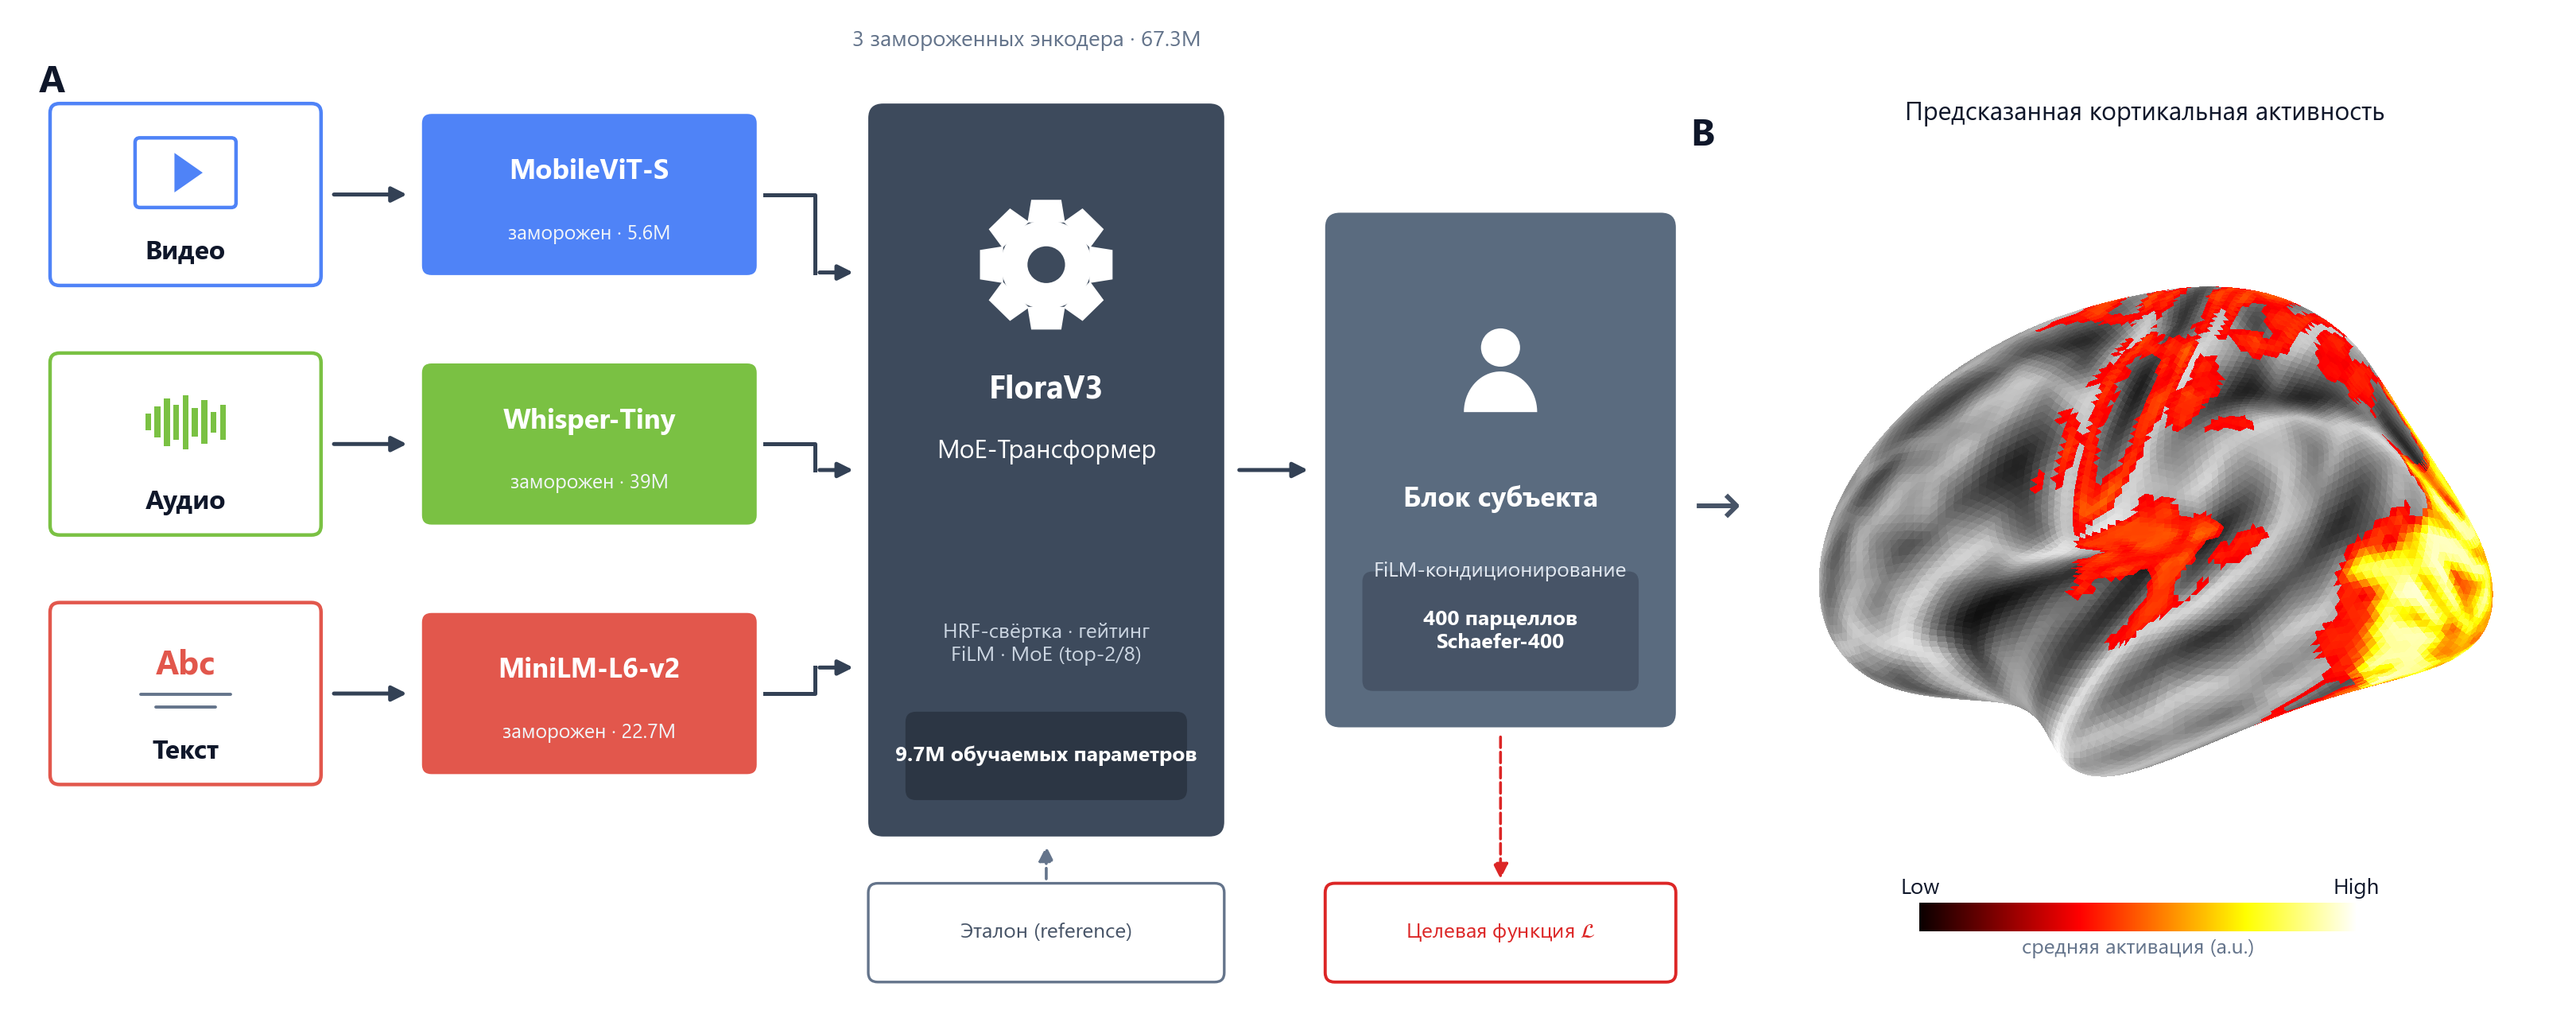
\includegraphics[width=0.78\textwidth]{assets/fig_overview.png}
\caption{Общая схема модели Flora}
\label{fig:overview}
\end{figure}

Дальше опишем нашу обучаемую часть блок за блоком.

\textbf{Проекторы.} Выходы трёх сетей имеют разный размер, 640 и 384.
Поэтому каждый поток сначала идёт через небольшую полносвязную сеть из
трёх слоёв. Она приводит всё к общему размеру. Ничего хитрого здесь
нет.

\textbf{Учёт движения.} Сеть для кадров смотрит на них по отдельности.
Она физически не может увидеть движение. А в фильме движение очень
важно. В мозге даже есть отдельная область для движущихся объектов. Мы
добавили к видеопотоку простую свёртку по времени. Она считает
разность соседних шагов. Так сеть получает сигнал «что изменилось».

\textbf{Перемешивание токенов.} Признаки трёх модальностей склеиваются
в одну последовательность. Порядок такой: кадр, звук, текст, снова
кадр, звук, текст и так далее. Тогда уже на первом слое трансформера
внимание может сравнивать «что видно» и «что слышно» в один и тот же
момент. Если бы потоки шли подряд, пришлось бы ждать последних слоёв.

\textbf{Трансформер со смесью экспертов.} Это ядро модели. Мы
остановились на двух слоях. Обычный блок полносвязной сети в них
заменён на смесь экспертов. Маленький роутер для каждого признака
выбирает двух специалистов из четырёх и смешивает их ответы. Интуиция
простая. Разные области коры реагируют на разное. Пусть разные подсети
специализируются на разном. Эксперты, правда, норовят сбиться в кучу.
Роутер нередко льёт всё на одного любимца. Поэтому добавлены два
штрафных слагаемых. Одно заставляет нагрузку распределяться ровно.
Второе не даёт роутеру выдавать слишком большие числа.

\textbf{Гемодинамическая задержка.} Это самое интересное место работы.
фМРТ измеряет BOLD-сигнал. Он не является самой активностью нейронов.
Это реакция кровотока на неё. Кровь реагирует с запаздыванием. Пик
приходится примерно на 5--6~секунд после стимула. Потом идёт медленный
спад с провалом около 12--16~секунд. Математически эту кривую хорошо
описывает так называемая двойная гамма-функция~[8]:
\begin{equation}
h(t) = \gamma(t;\, a_1{=}6,\, b_1{=}1) - \frac{1}{6}\,
\gamma(t;\, a_2{=}16,\, b_2{=}1),
\label{eq:hrf}
\end{equation}
где $\gamma(t; a, b)$ — гамма-распределение. Сама кривая показана на
рисунке~\ref{fig:hrf}. Выучивать эту задержку из 160 клипов мы сети не
стали. Заложили её в архитектуру заранее. Финальная часть модели —
свёртка по времени с ядром из восьми отсчётов, это около 12~секунд.
Инициализирована она кривой~\eqref{eq:hrf}. Во время обучения сеть
может немного подправить форму кривой. Но стартует она уже с
правильной. Похожая логика применена и в первых слоях внимания. Пары
событий, далёкие друг от друга по времени, получают штраф
$-\alpha|\Delta t|$, где $\alpha$ — обучаемый коэффициент.

\begin{figure}[H]
\centering
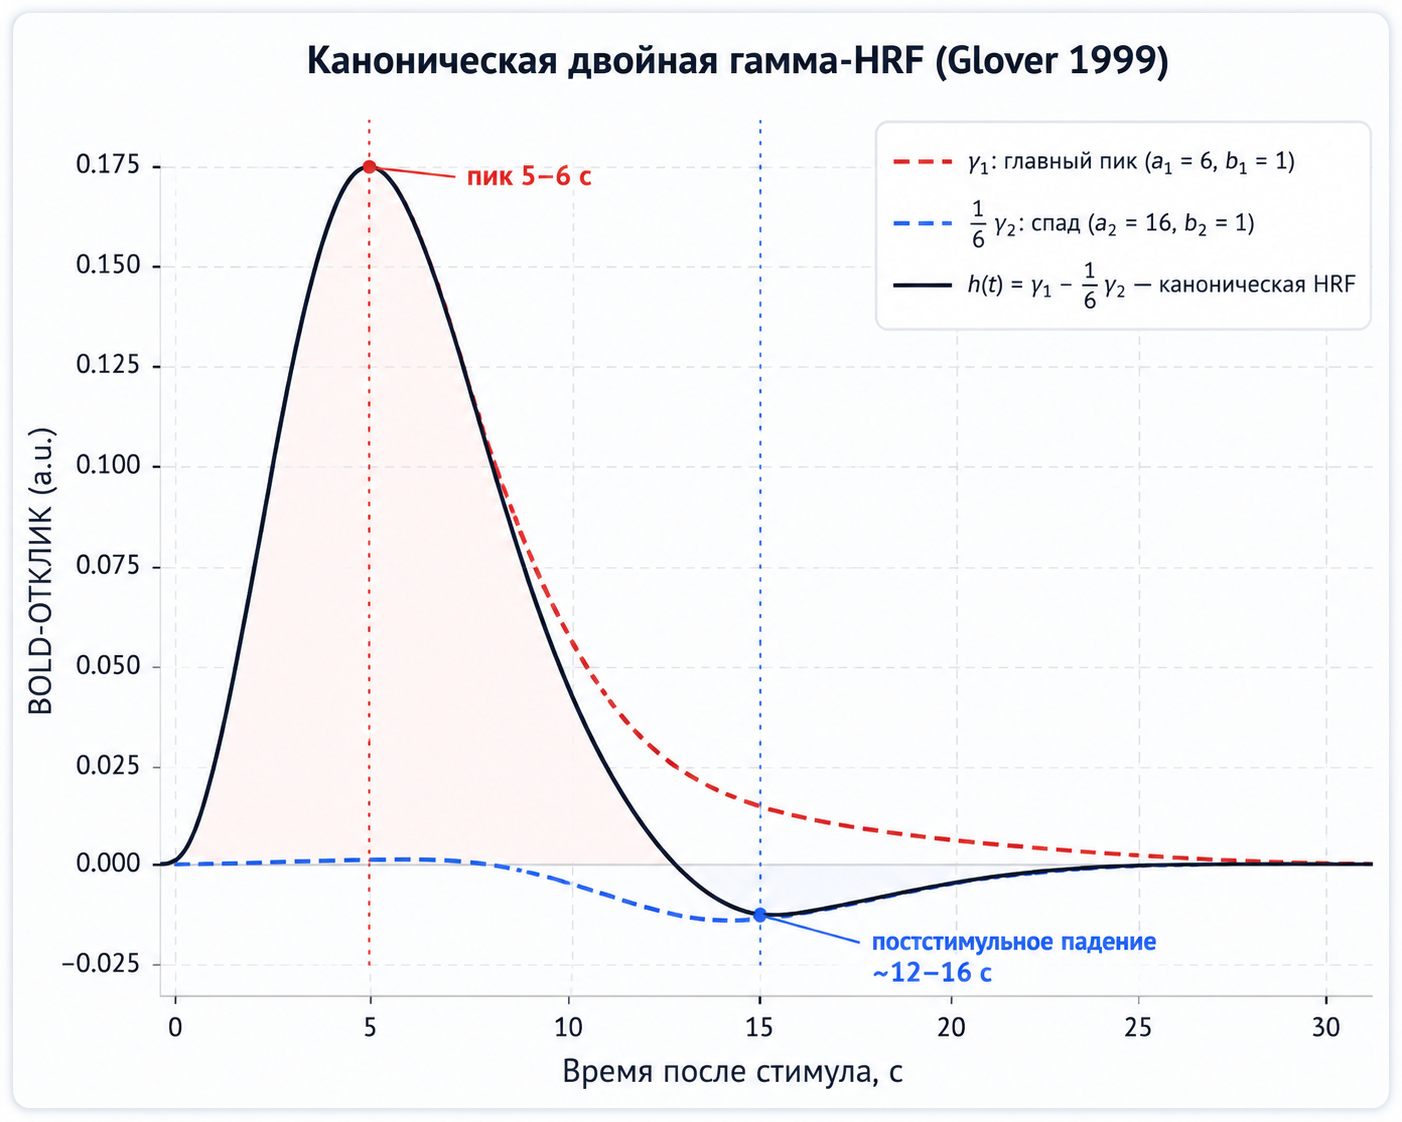
\includegraphics[width=0.7\textwidth]{assets/fig_hrf.png}
\caption{Кривая гемодинамического отклика: пик около 6 с и спад к 15--16 с}
\label{fig:hrf}
\end{figure}

\textbf{Гейтирование модальностей.} На каждом шаге у нас три токена:
видео, звук, текст. Можно было бы просто усреднить. Но это грубо.
Зрительной коре явно важнее видео, а речевым зонам — текст. Поэтому
модель учится взвешивать три модальности сама. Веса свои для каждого
момента времени.

\textbf{Выходная часть и подстройка под человека.} В конце стоит общий
полносвязный блок. Он выдаёт 400 чисел на каждый шаг, по одному на
каждую область коры. Для адаптации под конкретного человека мы сделали
вот что. К общему представлению добавляются два вектора, масштаб и
сдвиг. Они свои для каждого человека. Если бы на каждого человека
заводилась отдельная сеть, на 25 участников ушли бы десятки миллионов
лишних параметров. А так нужно 25\,600.

Итоговая архитектура целиком показана на рисунке~\ref{fig:arch}, а
распределение параметров — в таблице~\ref{tab:params} и на
рисунке~\ref{fig:budget}. Обучаемых параметров в опубликованной версии
— 9{,}7~млн. Для сравнения: в работах о моделях такого класса речь
обычно идёт о сотнях миллионов и миллиардах параметров.

\begin{figure}[H]
\centering
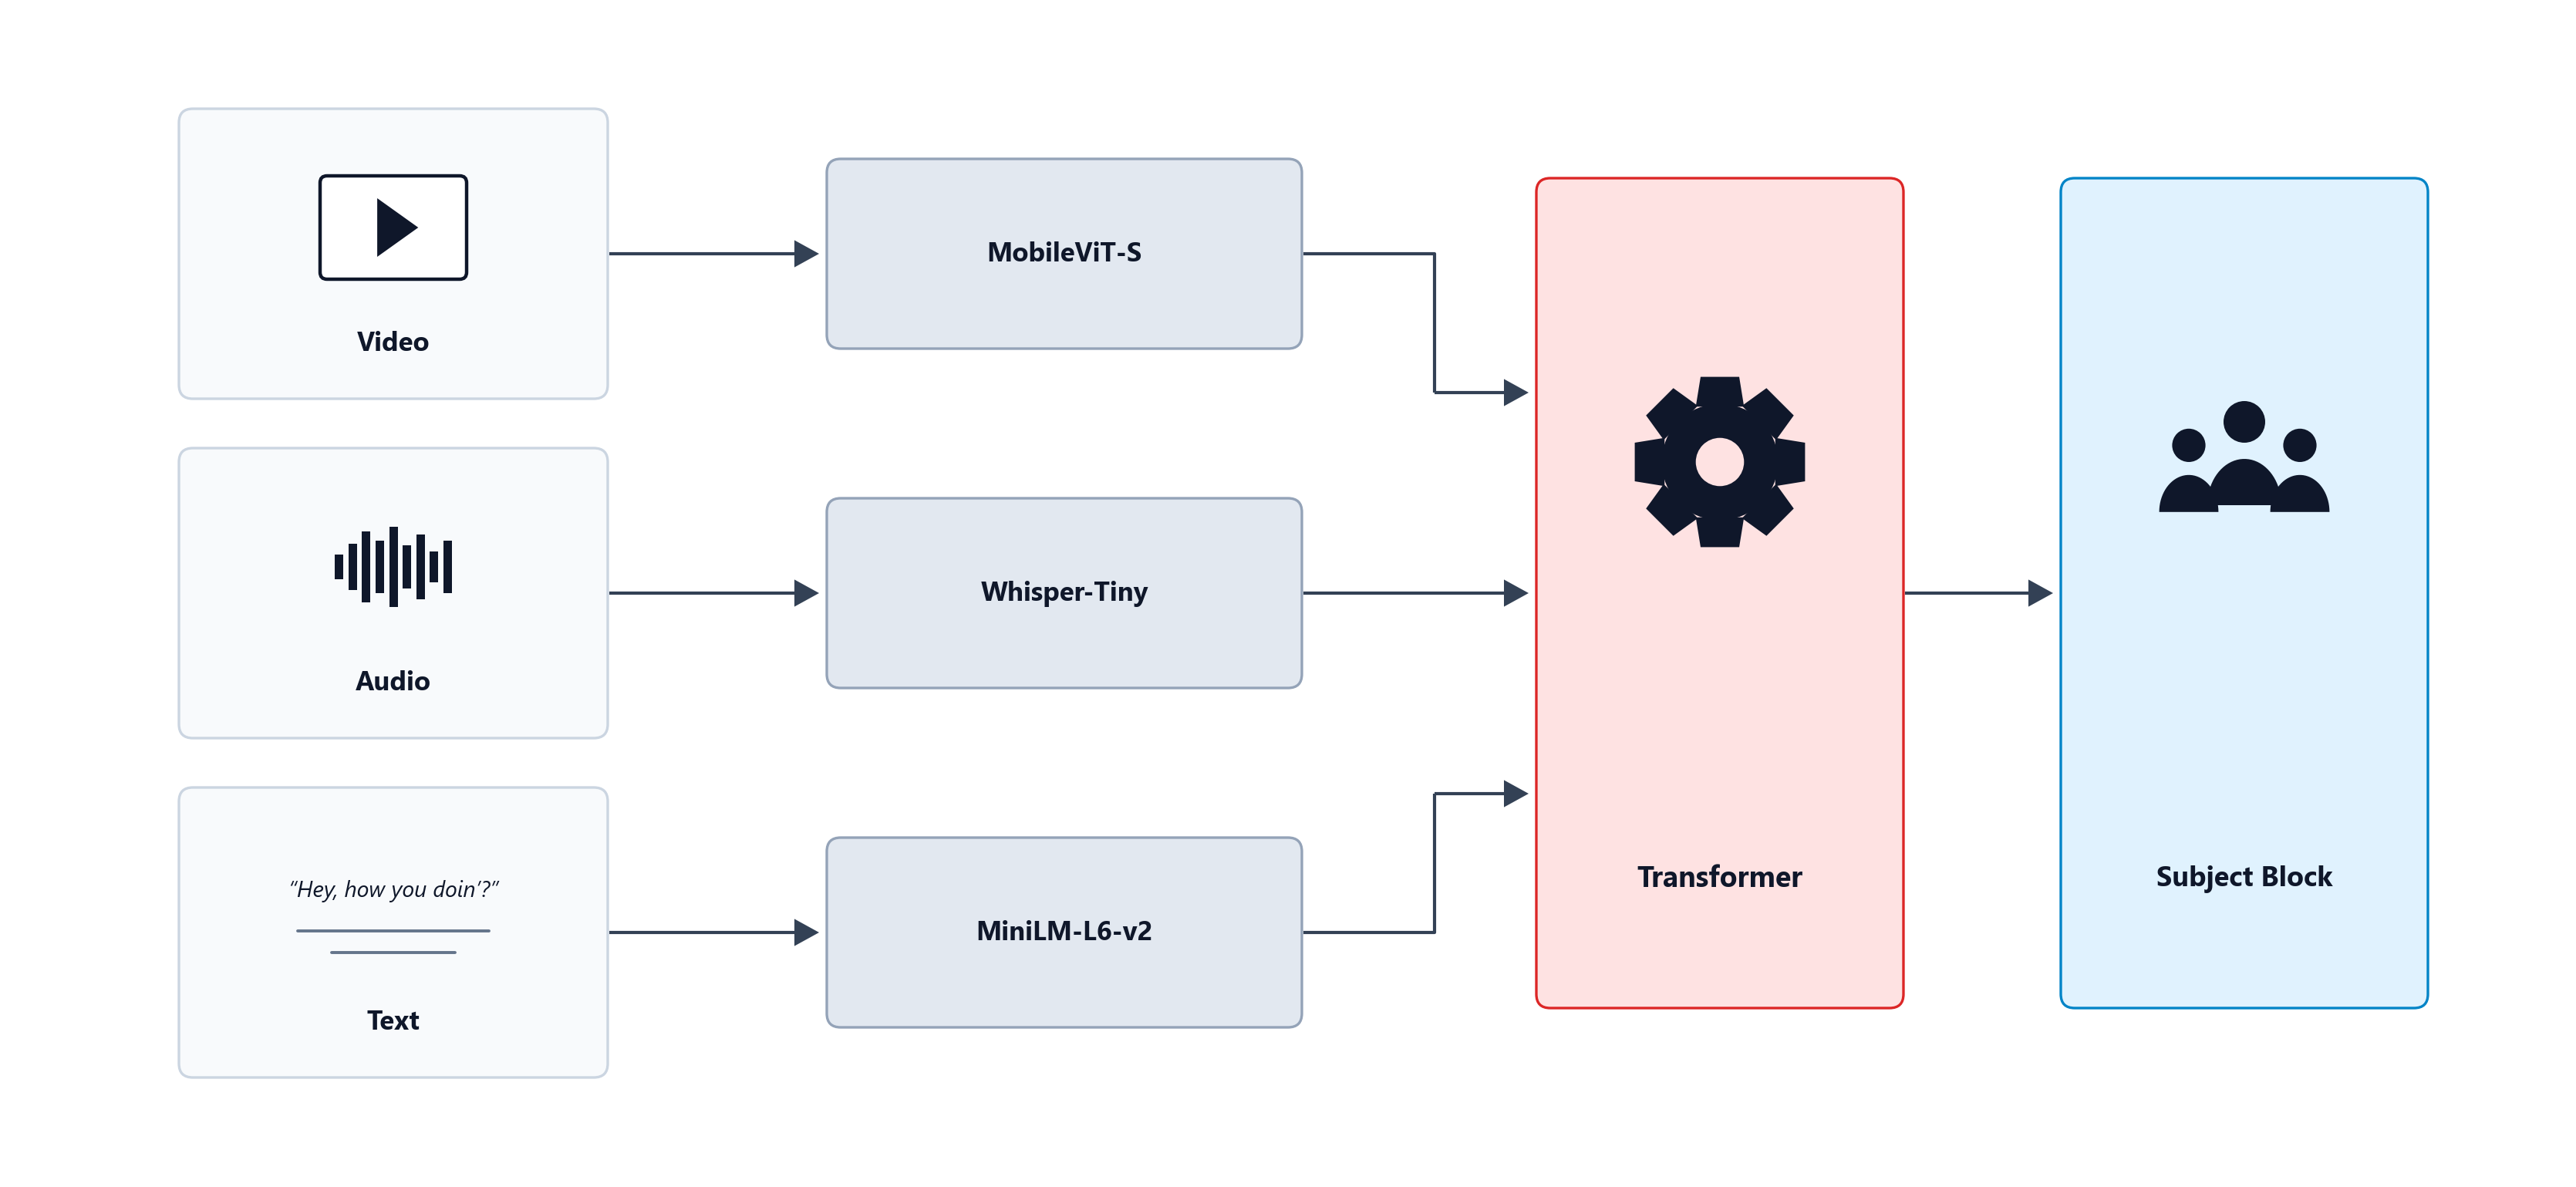
\includegraphics[width=0.85\textwidth]{assets/flora_architecture.png}
\caption{Архитектура модели Flora}
\label{fig:arch}
\end{figure}

\begin{figure}[H]
\centering
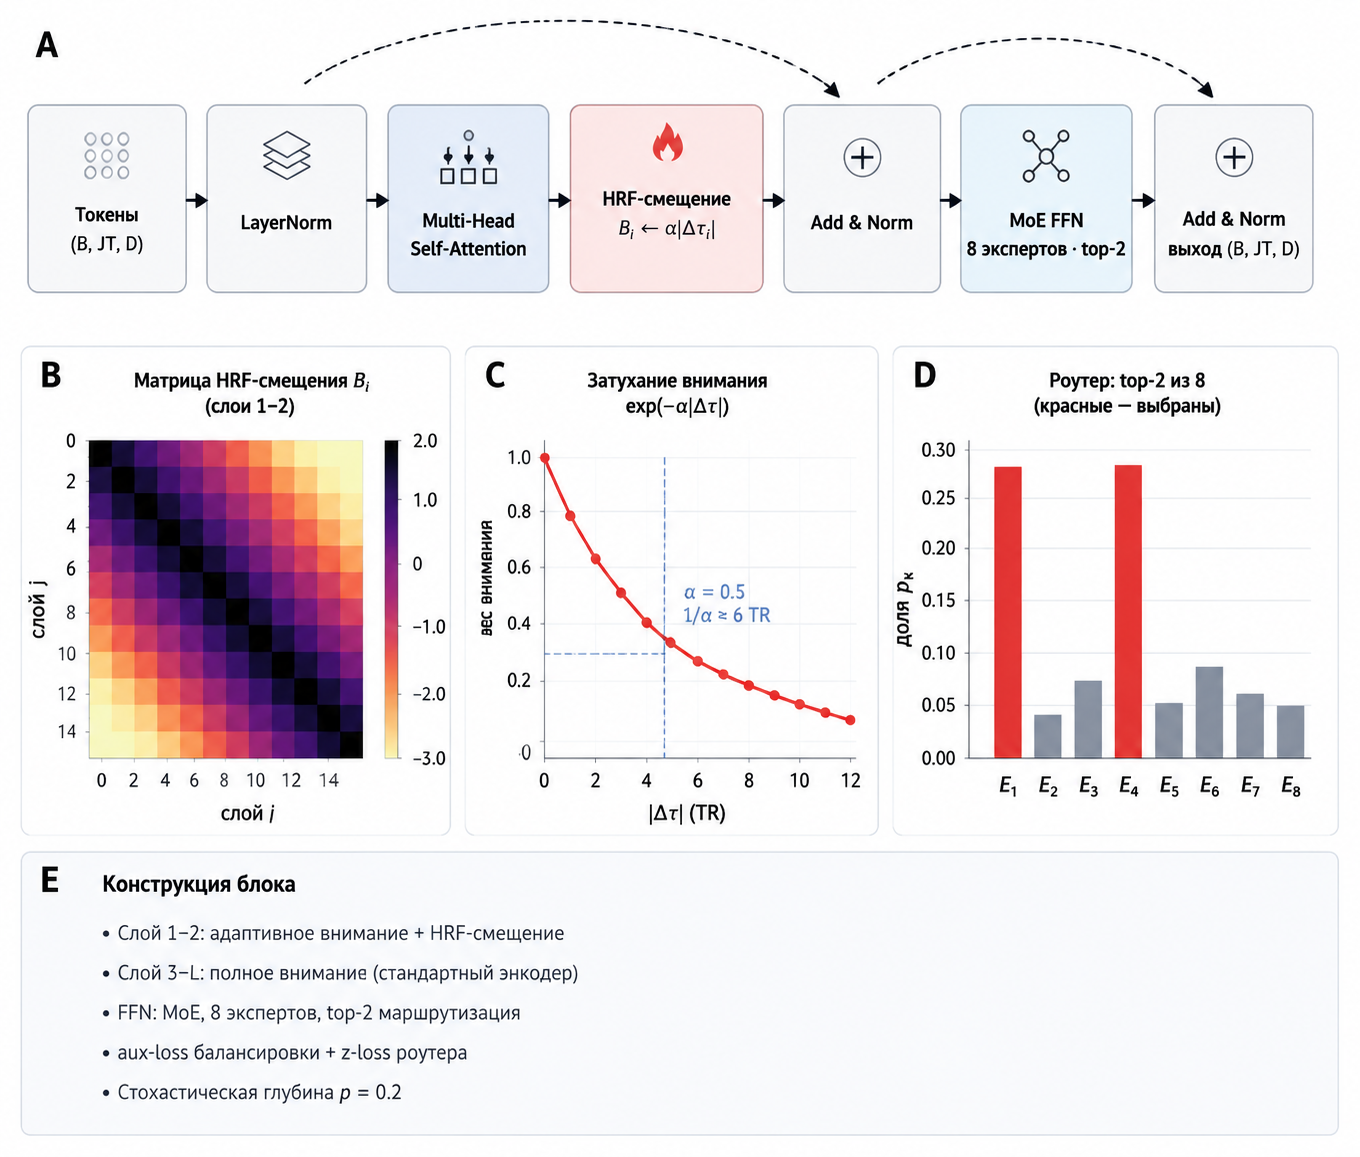
\includegraphics[width=0.9\textwidth]{assets/fig_moe_block.png}
\caption{Блок трансформера со смесью экспертов}
\label{fig:moe}
\end{figure}

\begin{table}[H]
\centering
\caption{Распределение параметров модели}
\label{tab:params}
\small
\begin{tabular}{lc}
\toprule
Компонент & Обучаемых параметров \\
\midrule
Проекторы трёх модальностей и учёт движения & $\sim$2{,}5 млн \\
Трансформер со смесью экспертов             & $\sim$9 млн \\
Гейтирование, свёртка HRF, эмбеддинги       & $\sim$0{,}4 млн \\
Выходная часть и подстройка под человека    & $\sim$2 млн \\
\midrule
\textbf{Всего обучается}                    & \textbf{9{,}7 млн} \\
Сети для признаков (вне обучения)           & 67{,}3 млн \\
\bottomrule
\end{tabular}
\end{table}

\begin{figure}[H]
\centering
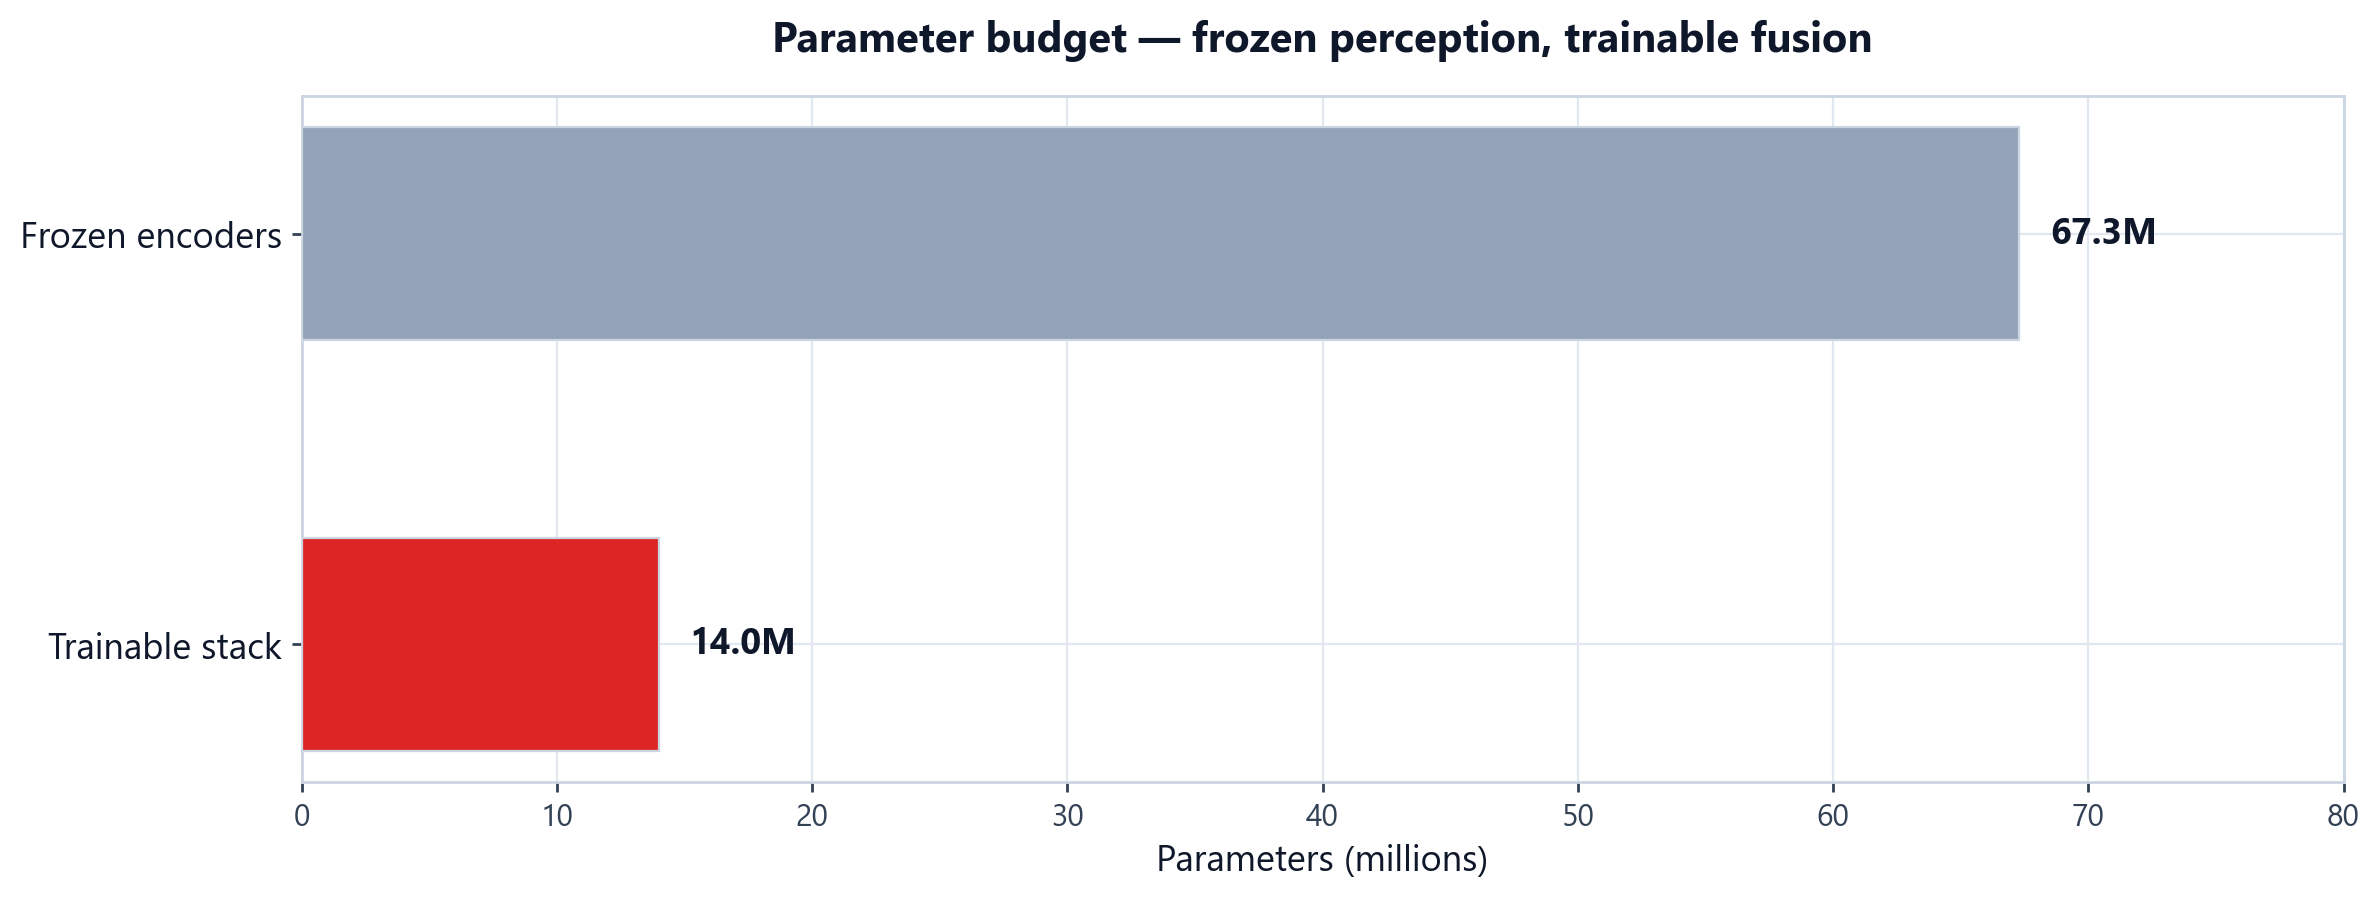
\includegraphics[width=0.85\textwidth]{assets/parameter_budget.png}
\caption{Соотношение обучаемой и вспомогательной частей модели}
\label{fig:budget}
\end{figure}

\subsection{Как мы обучали модель}

\textbf{Метрика качества.} Мы сравниваем предсказанный временной ряд с
тем, который указан в наборе данных. Сравнение идёт для каждой из 400
областей коры. Мера совпадения — корреляция Пирсона. Она равна 1 при
идеальном совпадении и 0, когда совпадения нет. Если ряды
противоположны, она уходит в минус:
\begin{equation}
r_v = \frac{\sum_i (\hat{y}_{v,i} - \bar{\hat{y}}_v)(y_{v,i} - \bar{y}_v)}
{\sqrt{\sum_i (\hat{y}_{v,i} - \bar{\hat{y}}_v)^2}\,
 \sqrt{\sum_i (y_{v,i} - \bar{y}_v)^2}},
\qquad
r = \frac{1}{400}\sum_{v=1}^{400} r_v .
\label{eq:pearson}
\end{equation}
Итоговая метрика $r$ — это среднее по всем 400 областям на 40
отложенных клипах.

\textbf{Функция потерь.} Основная часть — среднеквадратичная ошибка
между предсказанием и данными набора. Мы добавили к ней два
вспомогательных слагаемых. Первое штрафует за «дёрганость»
предсказаний во времени. Мозг не может менять активность скачками
каждые полторы секунды. Второе — та же ошибка, посчитанная на
прореженном сигнале. Оно нужно, чтобы модель не подгонялась под мелкий
шум:
\begin{equation}
\mathcal{L} = 0{,}60\,\mathrm{MSE}
+ 0{,}10\,\mathrm{TD}
+ 0{,}05\,\mathrm{MSE}_{\text{прореж.}}
+ 0{,}01\,\mathcal{L}_{\text{баланс}} .
\label{eq:loss}
\end{equation}

\textbf{Режим обучения.} Оптимизатор AdamW со скоростью обучения
$10^{-3}$. Три эпохи прогрева, дальше плавное затухание по косинусу.
Пакет из 16 клипов. Ограничение градиента 1{,}0. От переобучения
спасают dropout 0{,}3 и \emph{модальный} dropout. Второй работает так.
С вероятностью 0{,}5 во время обучения одна из модальностей случайно
выключается, но не все сразу. Без него модель быстро привыкала
опираться на одну модальность и заметно хуже переносилась на новые
клипы. Об этом мы уже писали выше. Основные параметры собраны в
таблице~\ref{tab:hyper}.

\begin{table}[H]
\centering
\caption{Основные параметры обучения}
\label{tab:hyper}
\small
\begin{tabular}{lc}
\toprule
Параметр & Значение \\
\midrule
Оптимизатор & AdamW, скорость обучения $10^{-3}$ \\
Размер пакета & 16 \\
Скрытая размерность / слои / головы & 256 / 2 / 4 \\
Экспертов / выбирается & 4 / 2 \\
Dropout / модальный dropout & 0{,}3 / 0{,}5 \\
Обучающие / проверочные клипы & 160 / 40 \\
Ранняя остановка & терпение 20 эпох \\
\bottomrule
\end{tabular}
\end{table}

Первые запуски мы делали вообще без ранней остановки. Просто гоняли
обучение подольше и смотрели на итог. Потом разобрали сохранённые
контрольные точки. Выяснилось, что лучшая осталась далеко позади, а
дальше качество только падало. Так появились и ранняя остановка, и
привычка сохранять лучшие точки. Об этом ещё будет речь дальше.

\textbf{Базовая модель для сравнения.} Результат имеет смысл только в
сравнении. Поэтому мы сами написали линейную ridge-регрессию. Она
получает те же самые признаки трёх модальностей, всего 1408 чисел на
шаг. По ним она учится предсказывать активность тех же 400 областей.
Параметров у неё всего 0{,}56~млн. Сравнение получается честным. Обе
модели видят одни и те же входные данные и проверяются на одних и тех
же 40 клипах.

\textbf{Что мы перепробовали.} С первого раза не заработало ничего. Об
этом стоит сказать отдельно. Иначе непонятно, откуда взялись числа,
которые стоят в таблицах дальше.

Самый первый вариант был совсем наивным. Мы усредняли признаки трёх
модальностей и подавали их в обычную полносвязную сеть. На обучающих
клипах всё выглядело прилично. А на проверочных корреляция держалась
около $0{,}2$. То есть сеть просто запоминала клипы.

Второй заход — трансформер на четыре слоя и восемь экспертов. Обучался
он дольше, а результат дал хуже. Роутер довольно быстро сваливался на
одного-двух экспертов, остальные почти не использовались. Два штрафа за
балансировку нагрузки помогли. Но с ними модель стала вести себя
слишком осторожно. В итоге мы вернулись к двум слоям и четырём
экспертам.

Третий провал был обиднее всего. Корреляция уже была приличной, но на
новых клипах проседала. Оказалось, сеть смотрит почти только на видео.
Звук и текст она игнорирует. По картинке она угадывала сюжет, и этого
хватало, чтобы пройти проверку. Вылечил это модальный dropout. Но
пришли мы к нему не сразу. Сначала перебрали разные штрафы за дисбаланс
модальностей.

Ещё две вещи дались не с первого раза. Инициализацию свёртки формой
кривой отклика мы сначала сделали случайной. Модель сходилась заметно
медленнее. Скорость обучения тоже пришлось подбирать вручную. При
$10^{-2}$ обучение расходилось, при $10^{-4}$ за отведённое время не
успевало сойтись.

\subsection{Результаты и их обсуждение}

\textbf{Динамика обучения.} Кривые показаны на
рисунке~\ref{fig:training}. На нулевой эпохе корреляция почти нулевая
($r = 0{,}033$). Модель ещё ничего не умеет. К 52-й эпохе она
дорастает до $r = 0{,}7278$, и это лучший результат за всё обучение.
Дальше началось то, чего мы сначала не ожидали. На обучающих клипах
метрика продолжает расти, а на проверочных — медленно падает. К 250-й
эпохе она опускается до $0{,}616$. То есть модель стала запоминать
конкретные клипы вместо общих закономерностей. Отсюда простой
практический вывод: 160 клипов — это впритык. И без аккуратного выбора
лучшей контрольной точки легко промахнуться.

\begin{figure}[H]
\centering
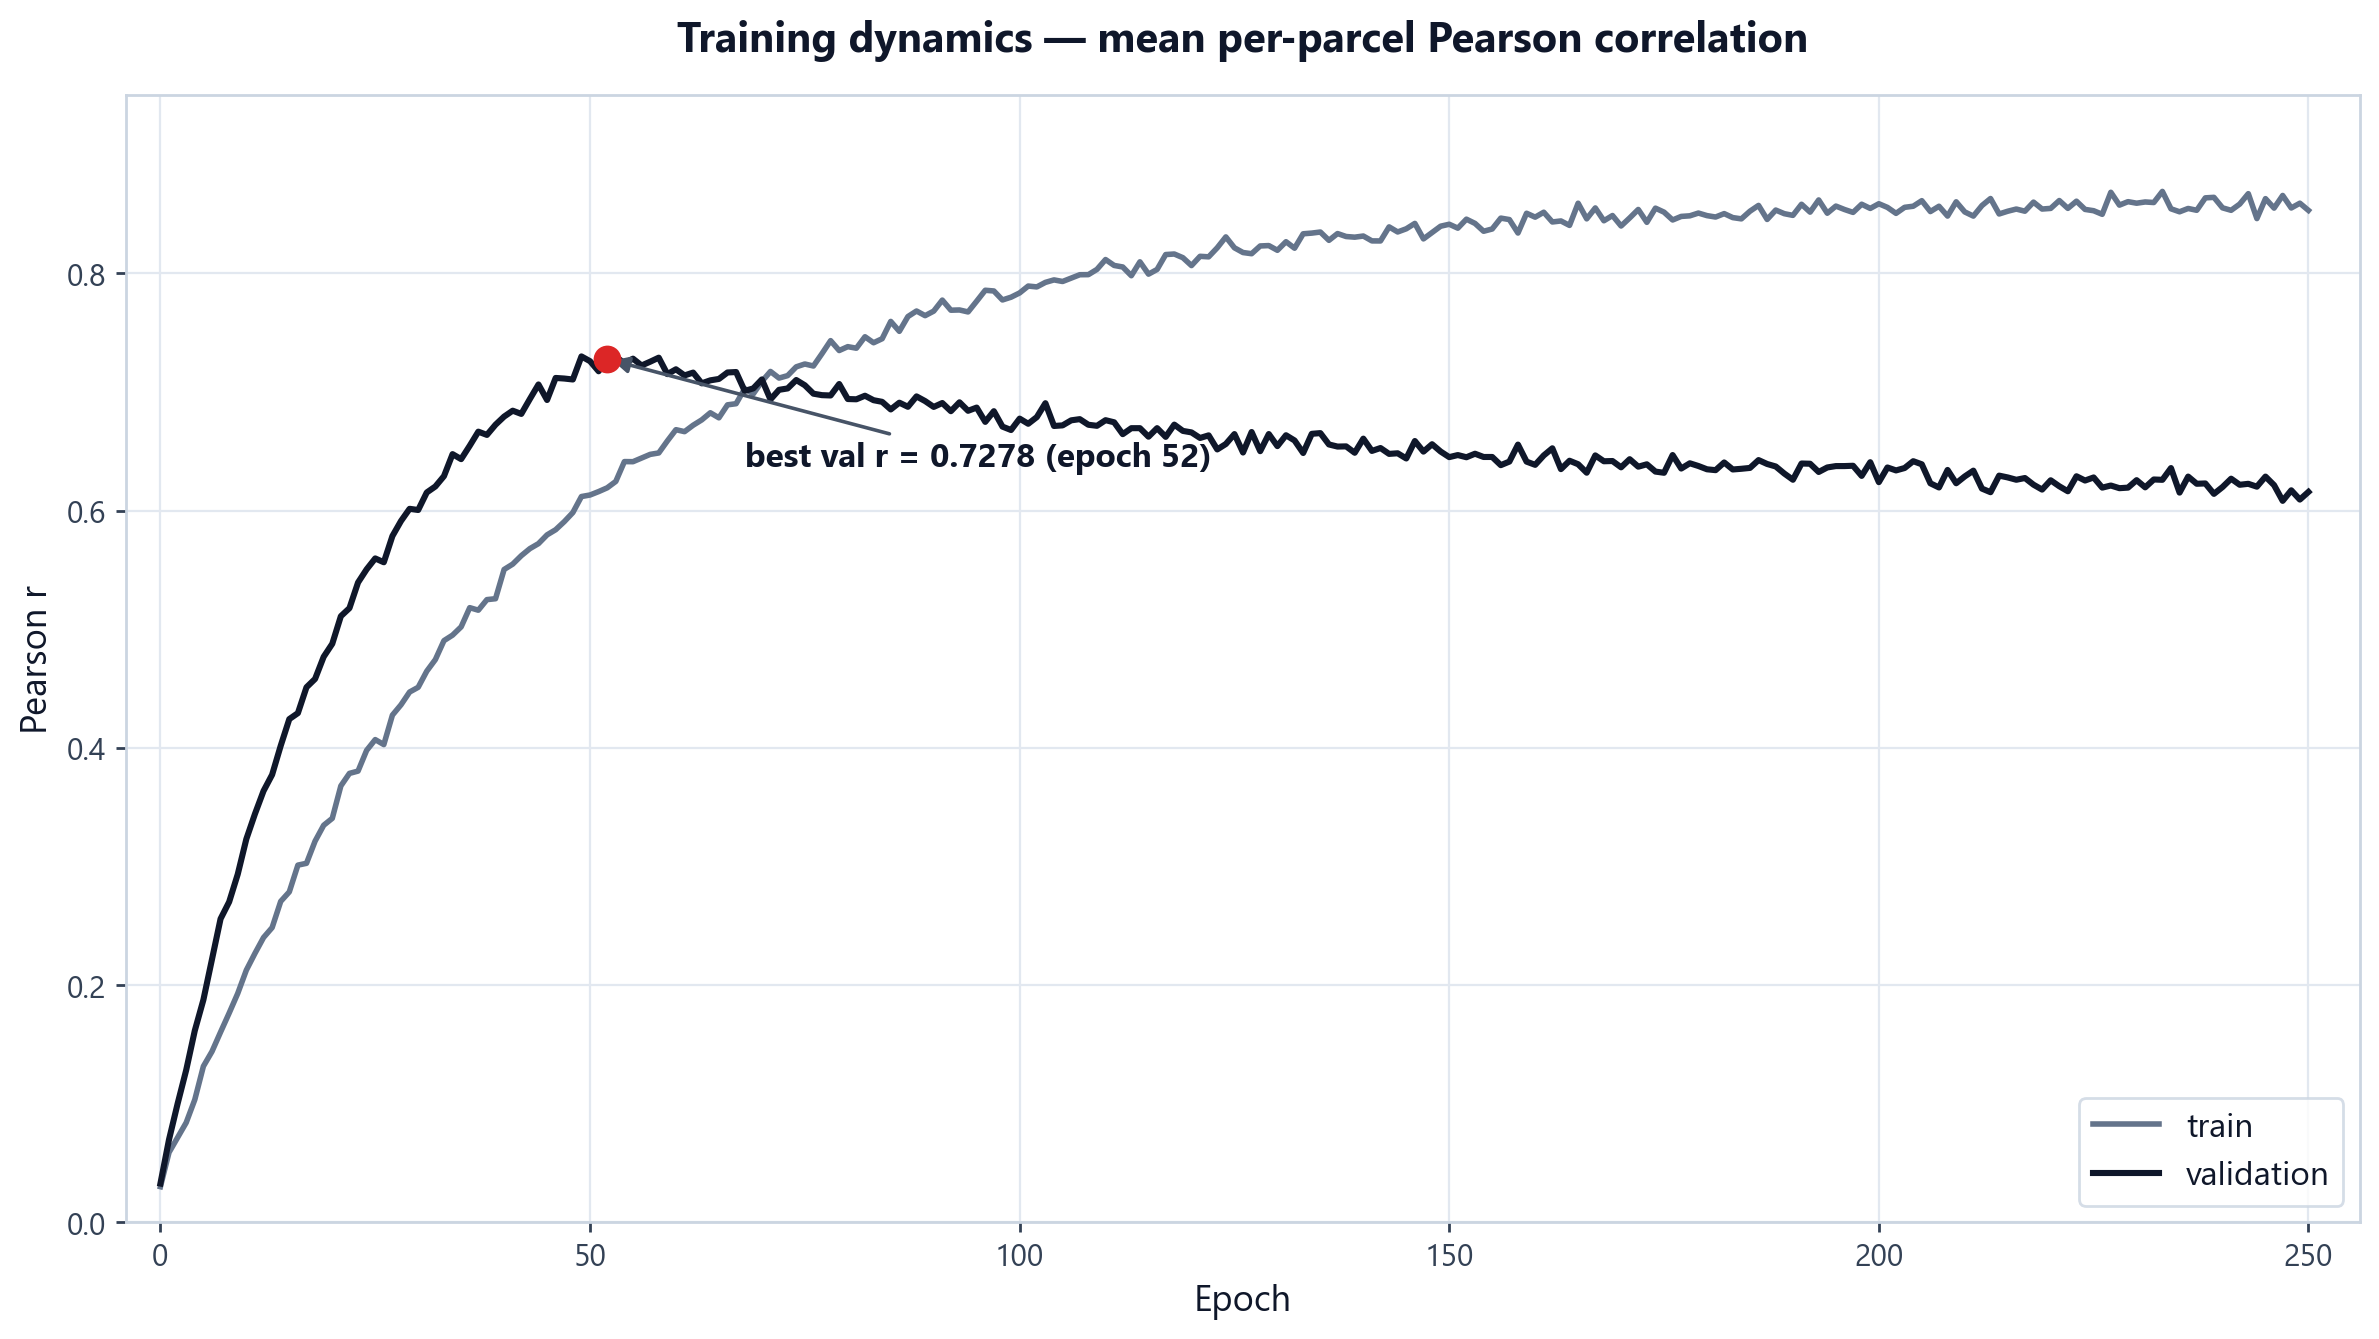
\includegraphics[width=0.9\textwidth]{assets/training_results.png}
\caption{Корреляция на обучающих и проверочных клипах по эпохам;
лучшая точка — эпоха 52}
\label{fig:training}
\end{figure}

\textbf{Сравнение с базовой моделью.} Итоговые цифры — в
таблице~\ref{tab:benchmark}. Наша модель со средним $r = 0{,}7278$
обходит линейную регрессию, у которой $0{,}3984$. Разница почти
двукратная. И это не эффект нескольких удачных областей. Почти по всей
коре Flora точнее линейной модели (рисунок~\ref{fig:hist}).

\begin{table}[H]
\centering
\caption{Сравнение моделей на 40 отложенных клипах}
\label{tab:benchmark}
\small
\begin{tabular}{lcc}
\toprule
Модель & Средняя корреляция $r$ & Параметров \\
\midrule
Константа (среднее по обучению) & 0{,}0000 & 0 \\
Линейная ridge-регрессия        & 0{,}3984 & 0{,}56 млн \\
\textbf{Flora}                  & \textbf{0{,}7278} & 9{,}7 млн \\
\bottomrule
\end{tabular}
\end{table}

\begin{figure}[H]
\centering
\begin{minipage}[t]{0.49\textwidth}
\centering
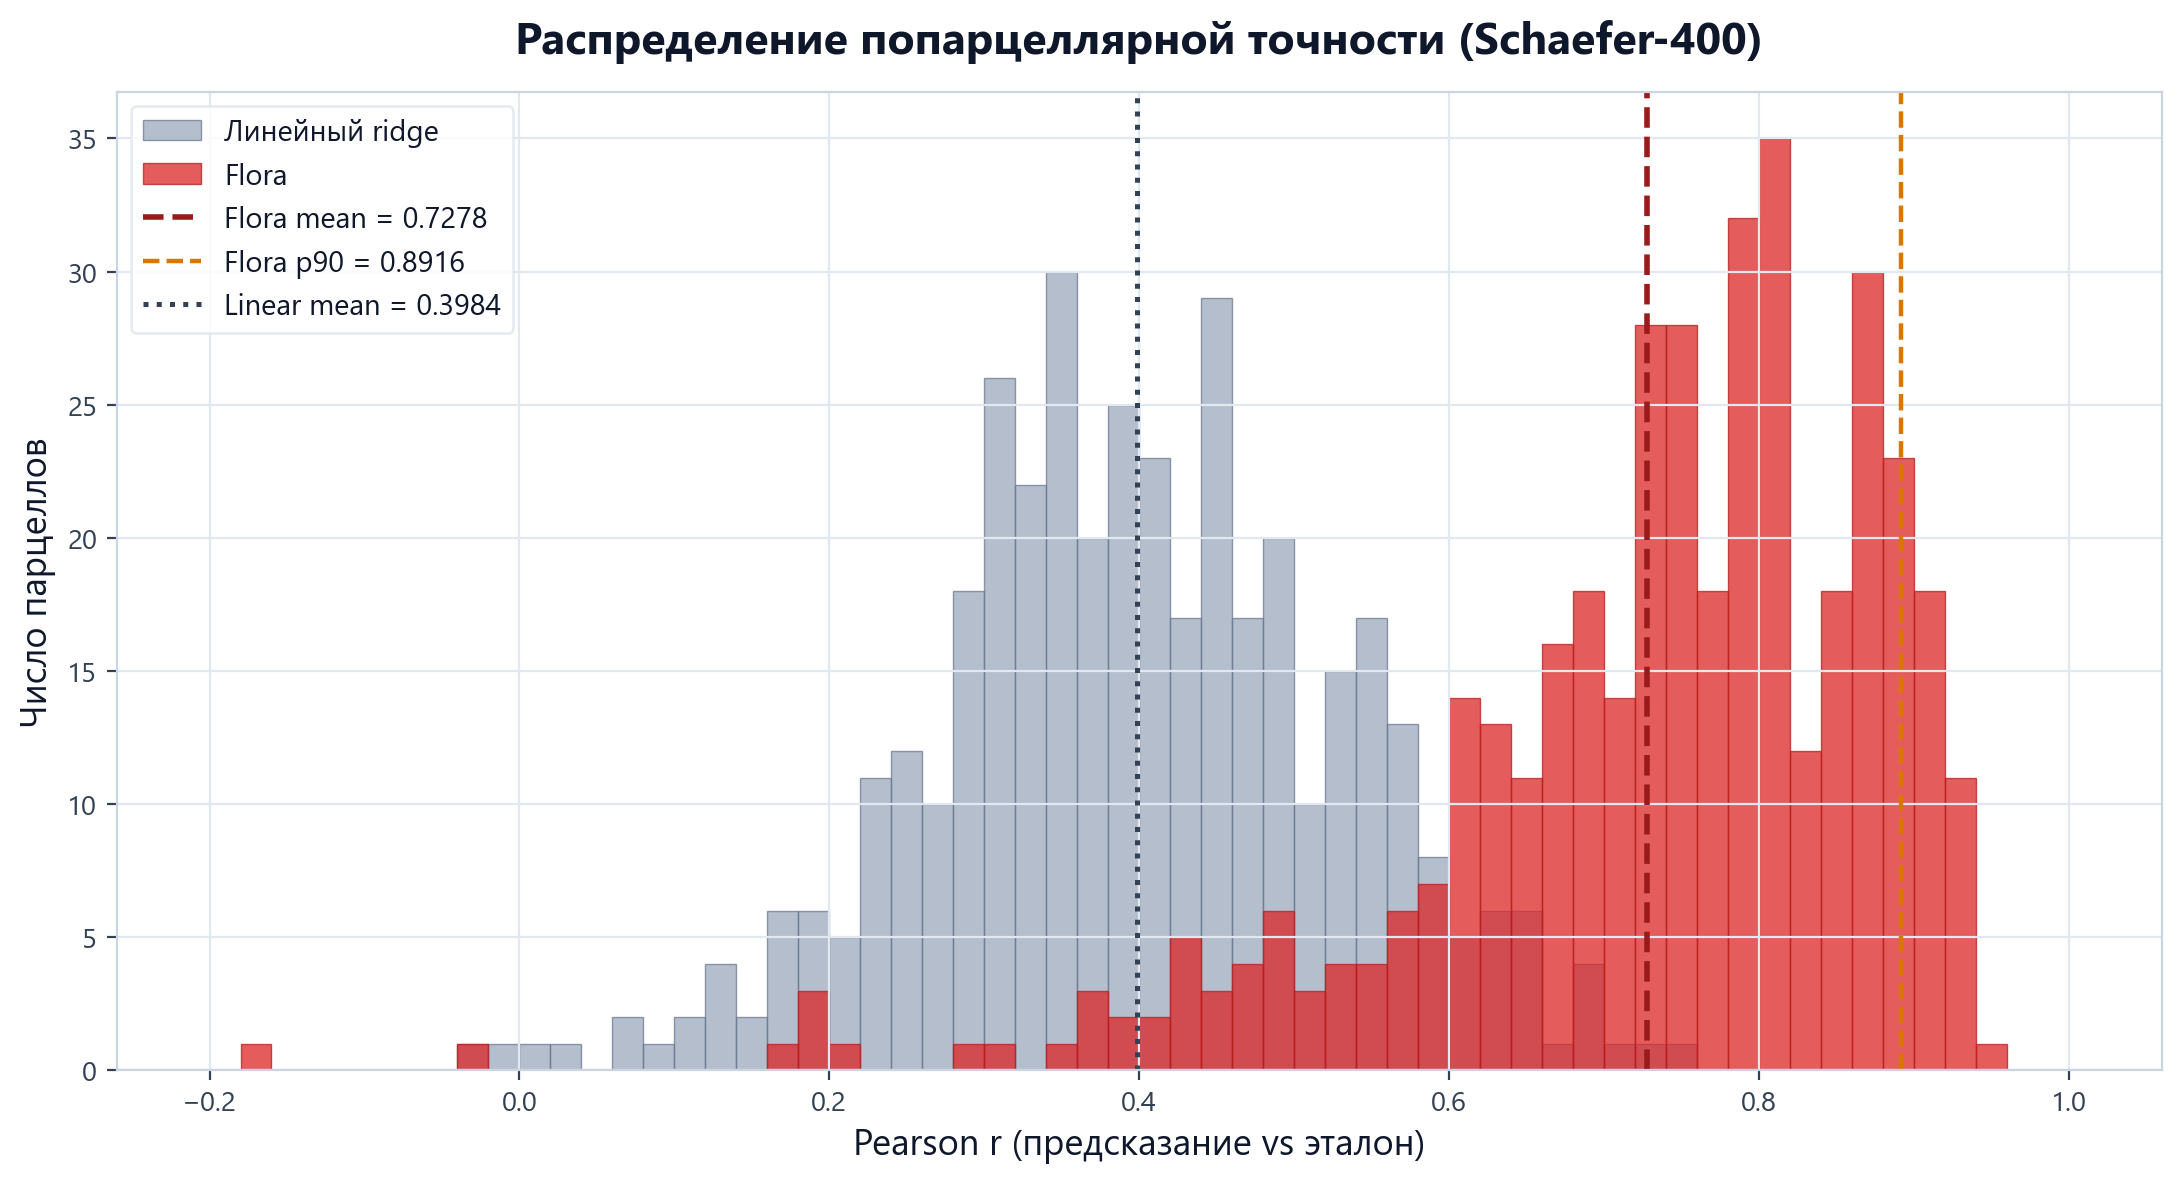
\includegraphics[width=0.9\textwidth]{benchmarks/figures/03_parcel_histogram.png}
\end{minipage}\hfill
\begin{minipage}[t]{0.49\textwidth}
\centering
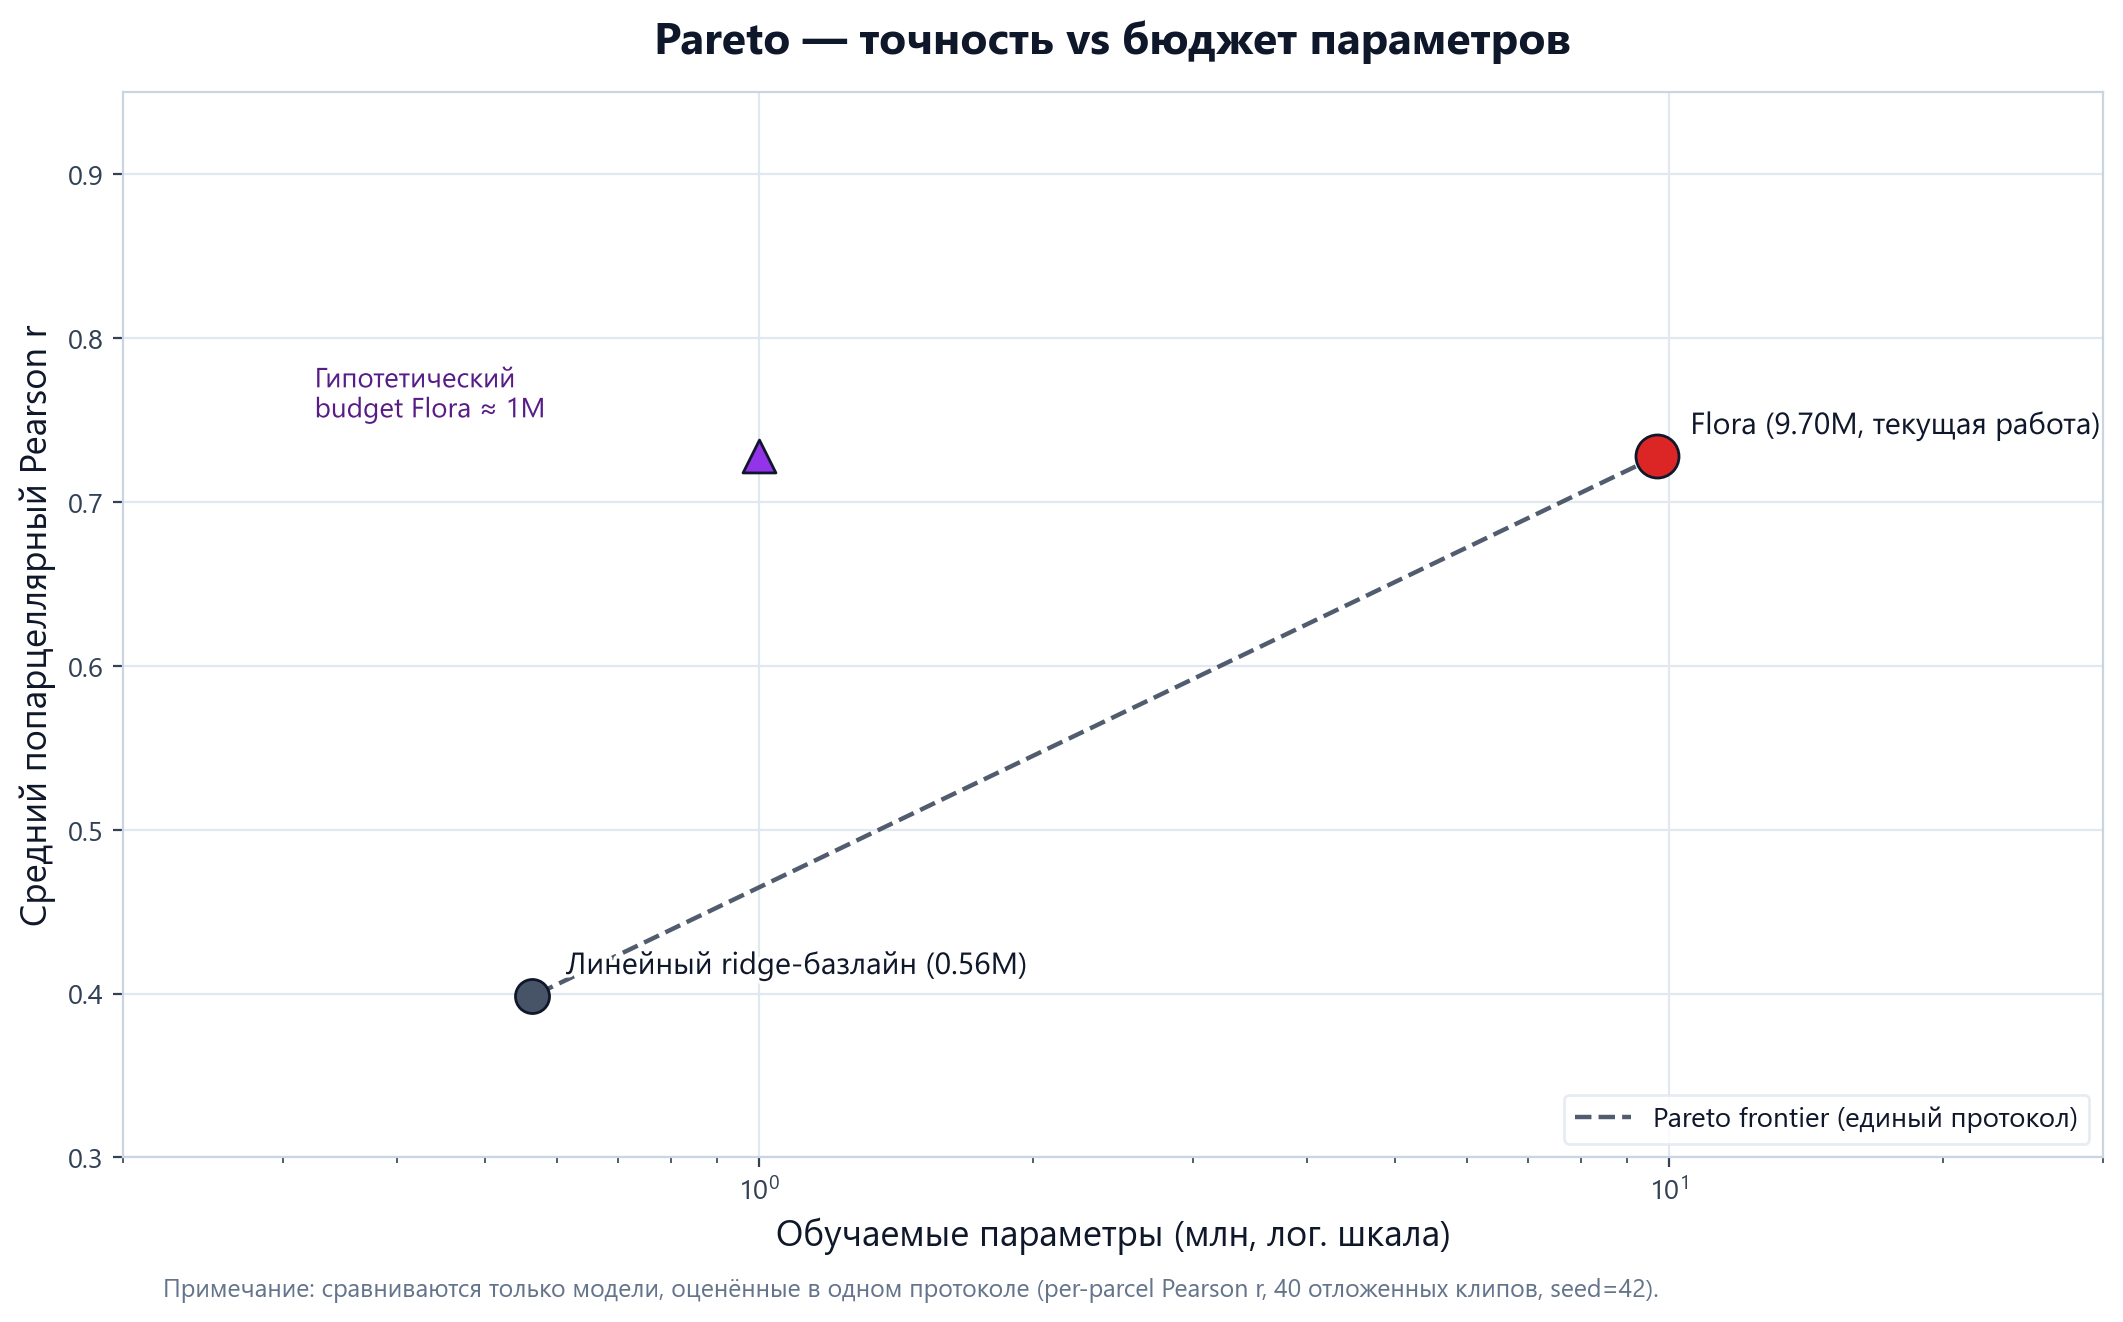
\includegraphics[width=0.9\textwidth]{benchmarks/figures/01_pareto_frontier.png}
\end{minipage}
\caption{Слева — распределение точности по 400 областям коры для Flora
и линейной модели; справа — соотношение «точность — размер модели»}
\label{fig:hist}
\end{figure}

Любопытная деталь. У линейной модели почти нет «плохих» областей,
разброс небольшой. Зато и хороших мало. Flora рискованнее. У неё есть
и области с $r > 0{,}9$, и пара областей с отрицательной корреляцией.
Худшая из них — $-0{,}31$. Медиана по областям — $0{,}76$.

\textbf{Какие области предсказываются лучше всего.} Мы разбили
результаты по семи функциональным сетям мозга
(таблица~\ref{tab:networks}). Результат нас сначала удивил. Лучше всего
предсказывается сеть пассивного режима (DMN, $r = 0{,}755$) и
лимбическая сеть ($0{,}746$). А зрительная кора — почти хуже всех
($0{,}701$). Казалось бы, мы подаём на вход видео. Почему зрение не на
первом месте? Разобравшись, мы нашли объяснение. DMN реагирует на смысл
происходящего. А смысл размазан по всем трём модальностям и по времени.
Наш трансформер с вниманием как раз хорошо ловит такие долгие
зависимости. Зрительная же кора реагирует на быстрые мелкие детали
картинки. Наш видеокодер работает с редкими кадрами и без явного
движения. Карта точности на поверхности мозга показана на
рисунке~\ref{fig:zones}. Самые точные области лежат в теменной и
префронтальной коре.

\begin{table}[H]
\centering
\caption{Точность предсказаний по функциональным сетям мозга}
\label{tab:networks}
\small
\begin{tabular}{lccc}
\toprule
Сеть & Областей & Flora & Линейная \\
\midrule
Пассивный режим (DMN) & 91 & 0{,}7550 & 0{,}4221 \\
Лимбическая           & 26 & 0{,}7456 & 0{,}4156 \\
Соматомоторная        & 77 & 0{,}7329 & 0{,}3974 \\
Дорсальное внимание   & 46 & 0{,}7290 & 0{,}4006 \\
Фронтопариетальная    & 52 & 0{,}7244 & 0{,}3977 \\
Зрительная            & 61 & 0{,}7009 & 0{,}3568 \\
Вентральное внимание  & 47 & 0{,}6943 & 0{,}3972 \\
\bottomrule
\end{tabular}
\end{table}

\begin{figure}[H]
\centering
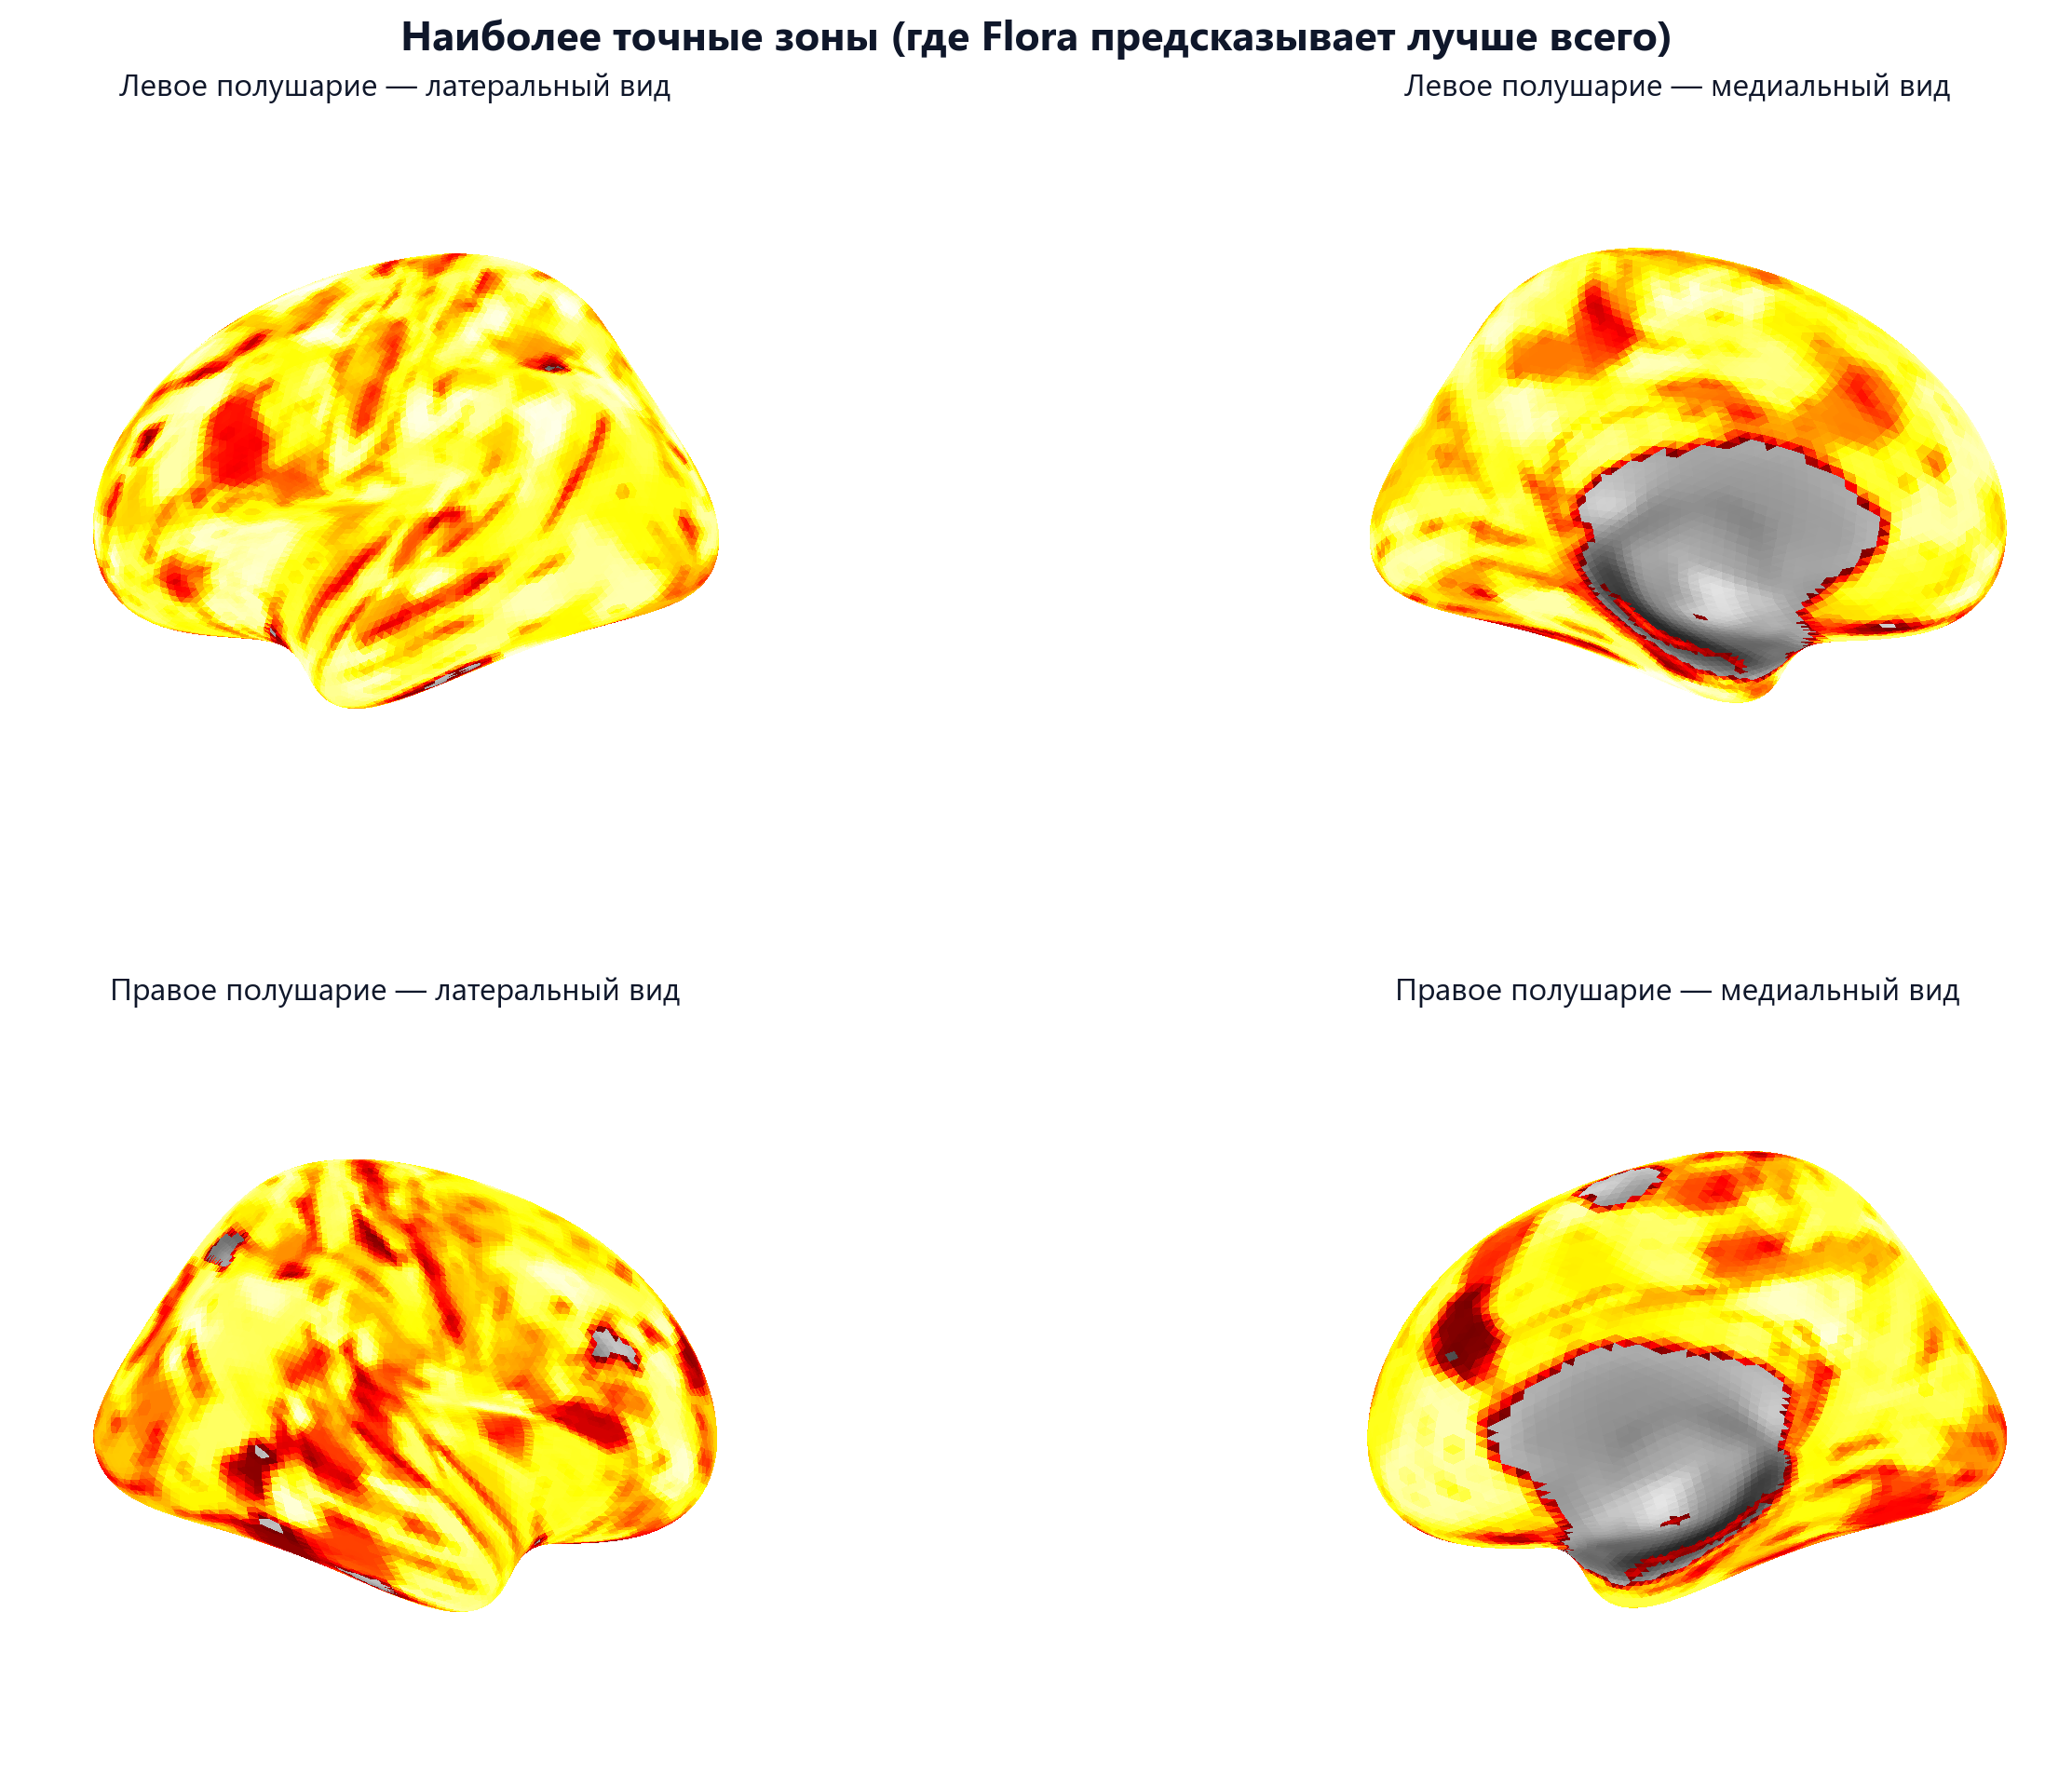
\includegraphics[width=0.85\textwidth]{benchmarks/figures/04_most_accurate_zones.png}
\caption{Точность предсказаний по областям коры на поверхности мозга}
\label{fig:zones}
\end{figure}

\textbf{Что получается на выходе.} Работу модели можно посмотреть
глазами. Предсказанную активность мы разворачиваем обратно: с 400
областей на всю поверхность мозга. Получаются карты. На
рисунке~\ref{fig:avg} — средняя активность при просмотре тестового
ролика. На рисунке~\ref{fig:temporal} — как картина меняется секунда за
секундой. Активность концентрируется в зрительной и височной коре. Для
видеостимула это ожидаемо.

\begin{figure}[H]
\centering
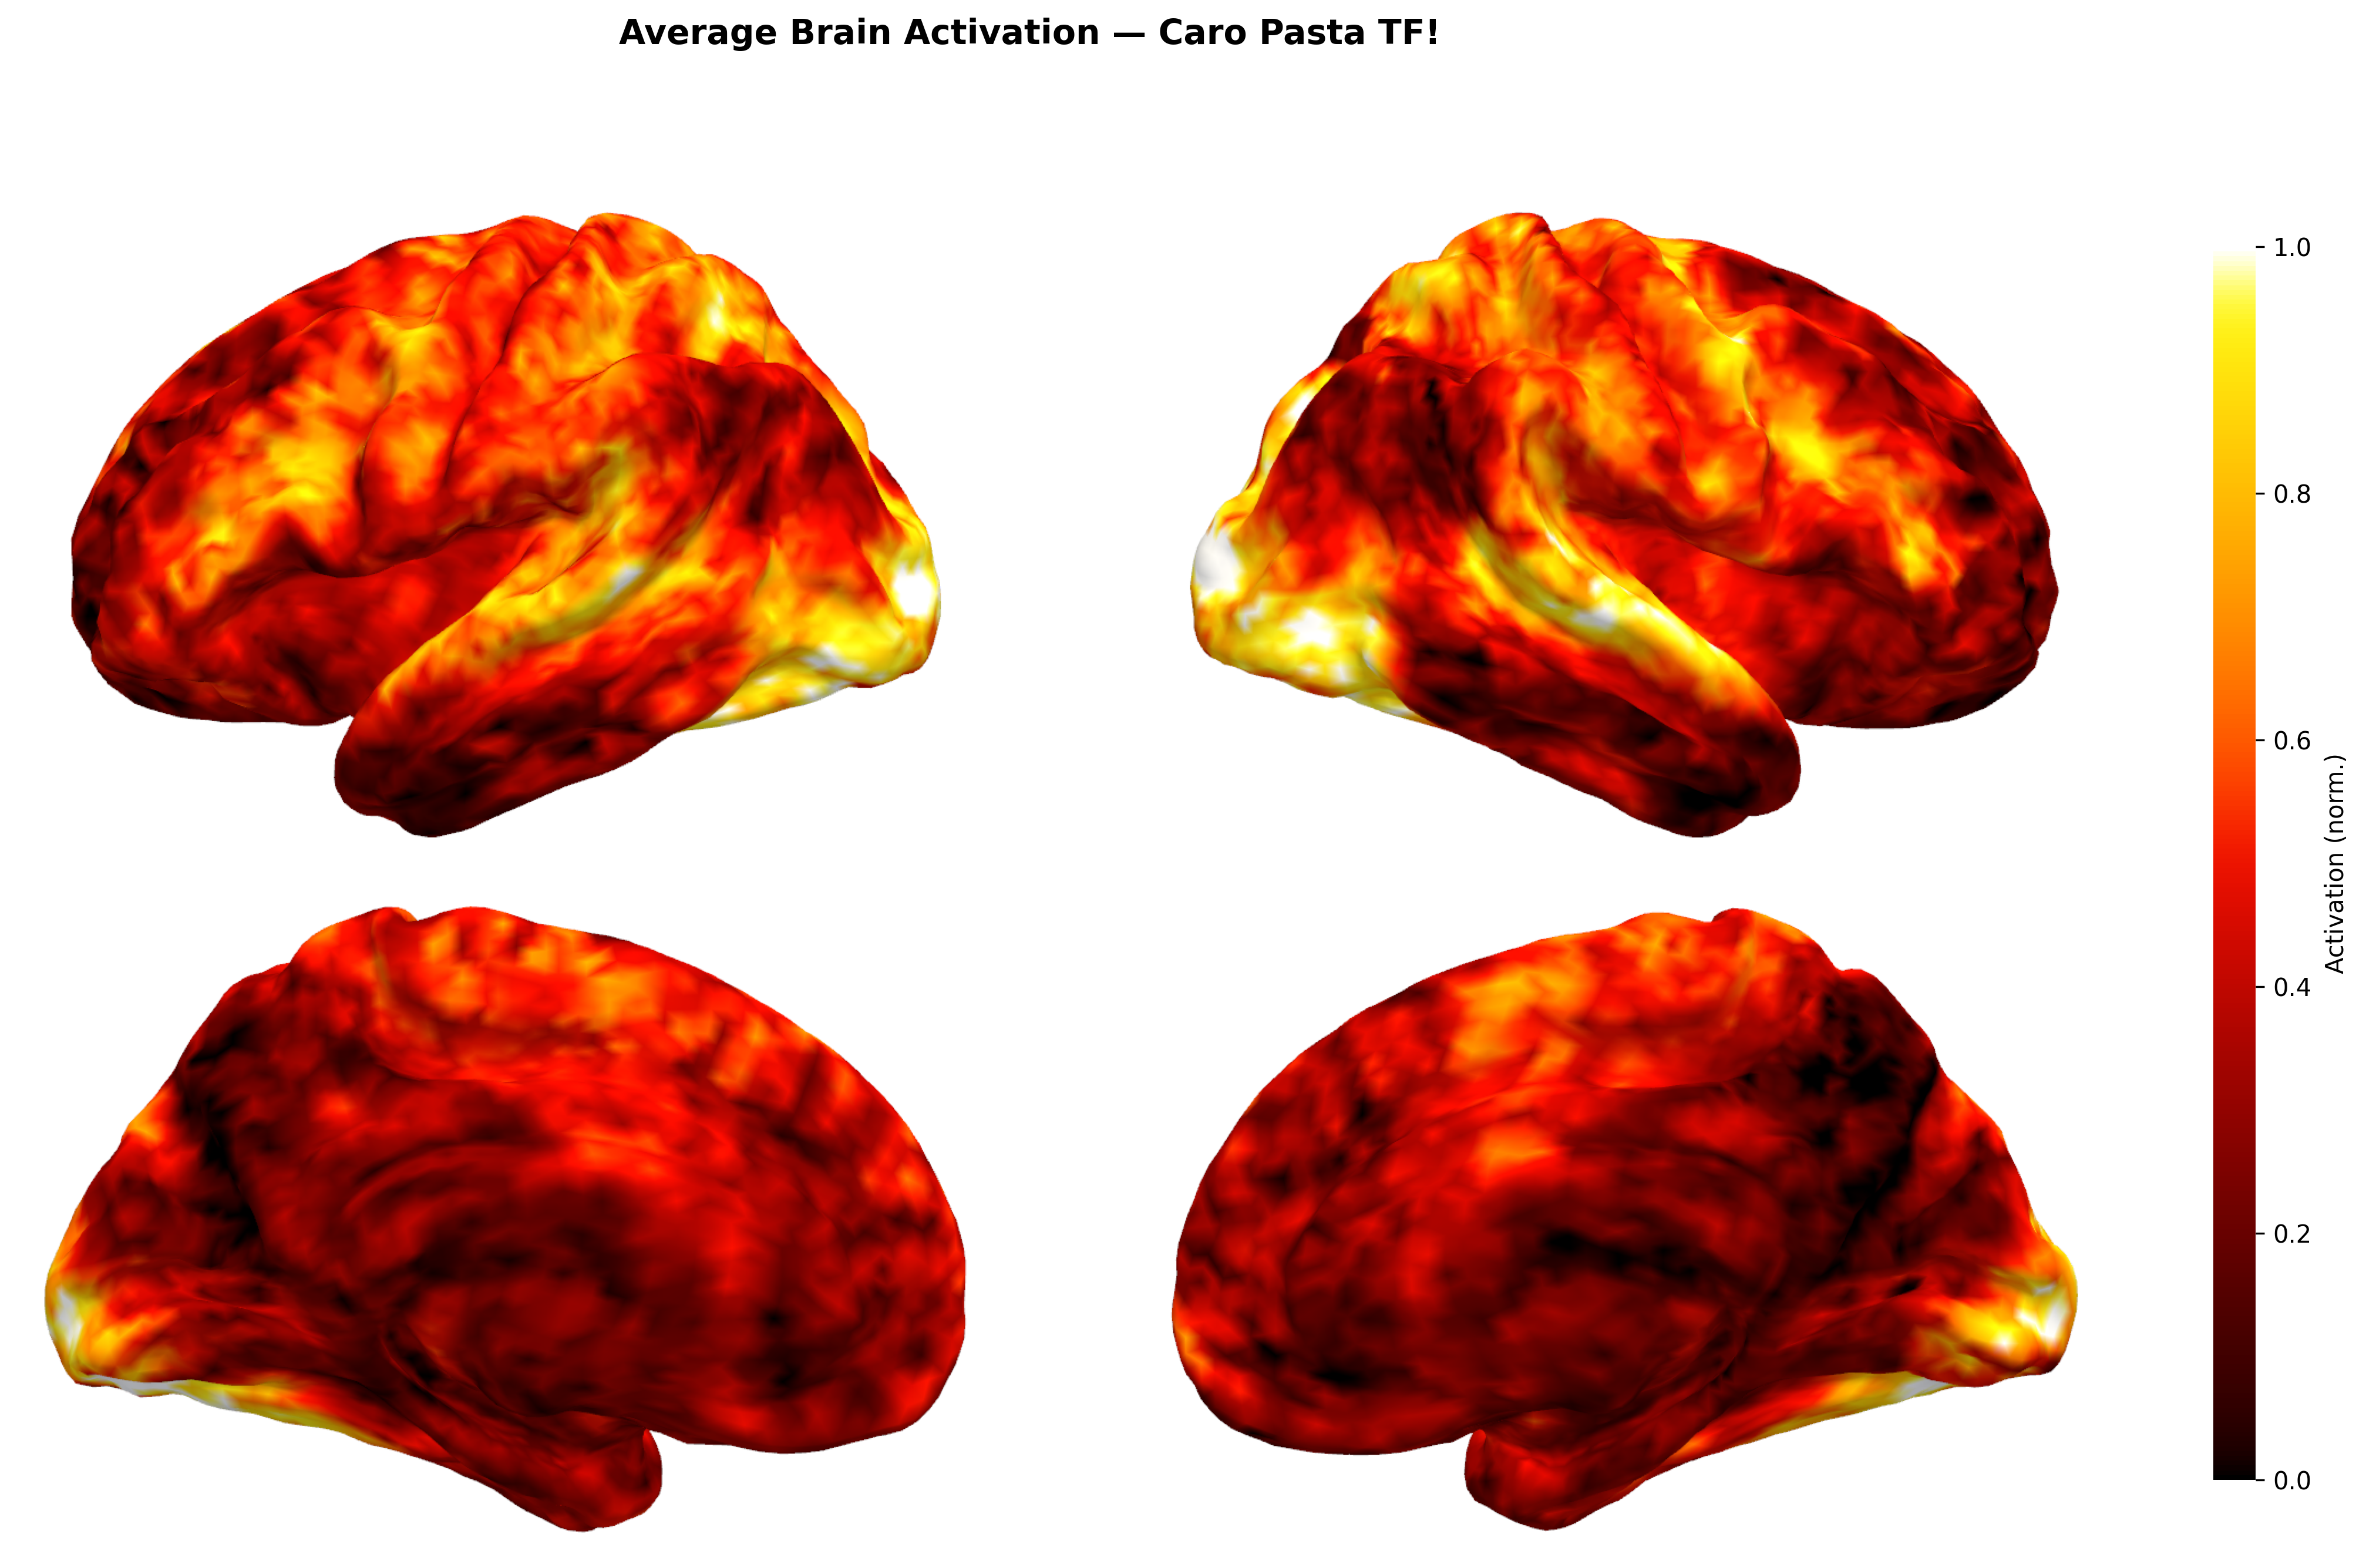
\includegraphics[width=0.9\textwidth]{assets/brain_avg_activation.png}
\caption{Средняя предсказанная активность коры при просмотре
тестового ролика (четыре проекции полушарий)}
\label{fig:avg}
\end{figure}

\begin{figure}[H]
\centering
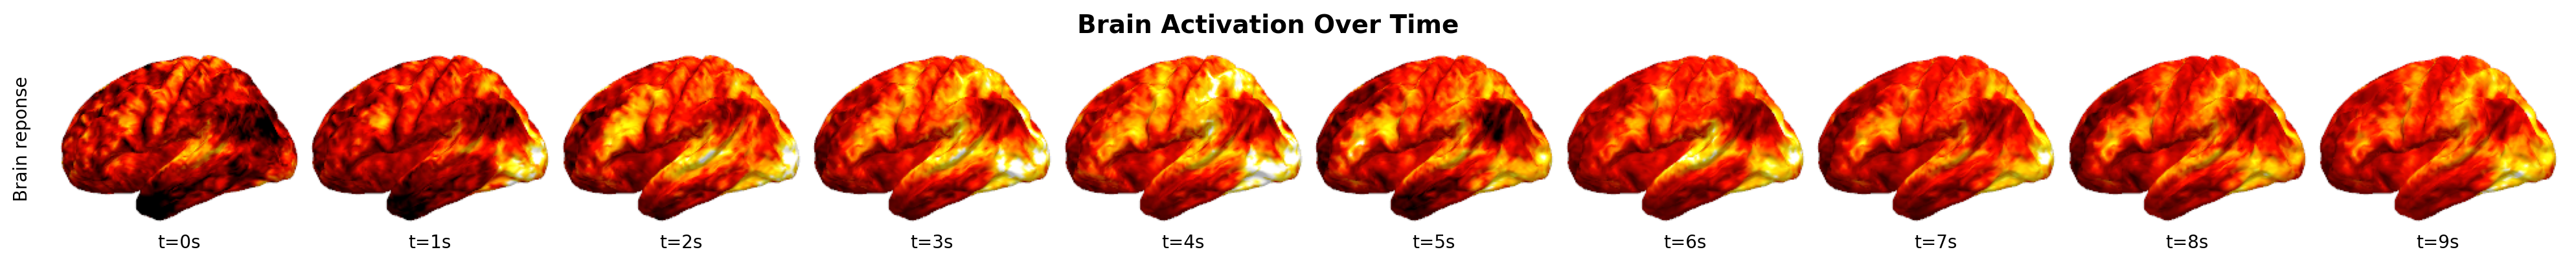
\includegraphics[width=0.85\textwidth]{assets/brain_temporal_sequence.png}
\caption{Изменение предсказанной активности от секунды к секунде}
\label{fig:temporal}
\end{figure}

\textbf{Чего мы не сделали.} Ограничения перечислим сразу. Пусть лучше
результат не выглядит больше, чем он есть.

Мы проверили модель на данных одного участника. Значит, всё, что
написано про «разных людей», пока остаётся возможностью архитектуры, а
не проверенным фактом. Дальше: у нас нет статистических тестов
значимости. Мы приводим только средние значения, а по отдельным
областям разброс большой. 160 обучающих клипов — это очень мало. Кривая
обучения это показывает: лучшая точка пришлась на 52-ю эпоху, дальше
качество только падало. Сравнивать Flora с большими моделями
кодирования напрямую мы не могли. Ни вычислительных мощностей, ни их
обучающих данных у нас нет. Поэтому единственная честная точка отсчёта
— линейная регрессия на тех же признаках. И последнее: сканы мы сами не
обрабатывали, а взяли готовые данные открытого набора.

Все эти пункты мы собираемся закрыть в следующей версии работы.

% ============================================================================
%  3. ЗАКЛЮЧЕНИЕ
% ============================================================================
\section{Заключение}

В работе получилась Flora. Это небольшая модель. Она берёт видеоролик
(картинка, звук, текст) и предсказывает, как меняется активность коры
головного мозга. Что удалось:

\begin{enumerate}
    \item Обучаемая часть — 9{,}7 млн параметров. Обучение заняло
          несколько часов на одном домашнем компьютере.
    \item На 40 отложенных клипах средняя корреляция вышла около
          $0{,}73$. У линейной регрессии на тех же признаках — $0{,}40$.
    \item Гипотеза в основном подтвердилась. Задержка и форма кривой
          отклика, заложенные заранее, действительно помогают маленькой
          сети. Выучивать это из 160 клипов ей было бы нечем.
    \item Выигрыш идёт по всей коре, а не за счёт нескольких удачных
          областей. Лучше всего предсказывается сеть пассивного
          режима, хуже всего — зрительная кора. Почему так вышло, мы
          разобрали в разделе~2.5.
\end{enumerate}

Практическая польза прежде всего в обучении. Модель и весь код
открыты: \url{https://github.com/qaddasd/Flora}.
На них можно показывать, как устроены модели кодирования мозга. Ни
сканера, ни кластера для этого не нужно.

Дальше мы хотим обучить модель на настоящих данных фМРТ. Ещё —
провести контрольные эксперименты без отдельных блоков (свёртка HRF,
смесь экспертов, подстройка под человека). Хотим добавить
статистическую проверку и взять ещё один открытый корпус.

% ============================================================================
%  СПИСОК ИСПОЛЬЗОВАННЫХ ИСТОЧНИКОВ
% ============================================================================
\renewcommand{\refname}{Список использованных источников}
\begin{thebibliography}{14}
\addcontentsline{toc}{section}{Список использованных источников}
\small\singlespacing

\bibitem{logothetis} Logothetis~N.K. What we can do and what we cannot
do with fMRI // Nature. — 2008. — Vol.~453. — P.~869–878.

\bibitem{cinebrain} Gao~J., Liu~Y., Yang~B., Feng~J., Fu~Y. CineBrain:
A large-scale multi-modal brain dataset during naturalistic
audiovisual narrative processing // arXiv preprint arXiv:2503.06940. —
2025. — URL: https://github.com/onepunchmonk/cine-brain.

\bibitem{kay} Kay~K.N., Naselaris~T., Prenger~R.J., Gallant~J.L.
Identifying natural images from human brain activity // Nature. —
2008. — Vol.~452. — P.~352–355.

\bibitem{mitchell} Mitchell~T.M., Shinkareva~S.V., Carlson~A. et al.
Predicting human brain activity associated with the meanings of nouns
// Science. — 2008. — Vol.~320, №~5880. — P.~1191–1195.

\bibitem{naselaris} Naselaris~T., Kay~K.N., Nishimoto~S., Gallant~J.L.
Encoding and decoding in fMRI // NeuroImage. — 2011. — Vol.~56, №~2. —
P.~400–410.

\bibitem{huth} Huth~A.G., de~Heer~W.A., Griffiths~T.L., Theunissen~F.E.,
Gallant~J.L. Natural speech reveals the semantic maps that tile human
cerebral cortex // Nature. — 2016. — Vol.~532. — P.~453–458.

\bibitem{wen} Wen~H., Shi~J., Zhang~Y. et al. Neural encoding and
decoding with deep learning for dynamic natural vision // Cerebral
Cortex. — 2018. — Vol.~28, №~12. — P.~4136–4160.

\bibitem{glover} Glover~G.H. Deconvolution of impulse response in
event-related BOLD fMRI // NeuroImage. — 1999. — Vol.~9, №~4. —
P.~416–429.

\bibitem{lindquist} Lindquist~M.A., Geuter~S., Wager~T.D., Caffo~B.S.
Modelling the hemodynamic response function in fMRI: efficiency, bias,
and mis-modeling // NeuroImage. — 2019. — Vol.~189. — P.~187–198.

\bibitem{esteban} Esteban~O., Markiewicz~C.J., Blair~R.W. et al.
fMRIPrep: a robust preprocessing pipeline for functional MRI // Nature
Methods. — 2019. — Vol.~16, №~1. — P.~111–116.

\bibitem{fischl} Fischl~B. FreeSurfer // NeuroImage. — 2012. —
Vol.~62, №~2. — P.~774–781.

\bibitem{schaefer} Schaefer~A., Kong~R., Gordon~E.M. et al.
Local-global parcellation of the human cerebral cortex from intrinsic
functional connectivity MRI // Cerebral Cortex. — 2018. — Vol.~28,
№~9. — P.~3095–3114.

\bibitem{yeo} Yeo~B.T.T., Krienen~F.M., Sepulcre~J. et al. The
organization of the human cerebral cortex estimated by intrinsic
functional connectivity // Journal of Neurophysiology. — 2011. —
Vol.~106, №~3. — P.~1125–1165.

\bibitem{nilearn} Abraham~A., Pedregosa~F., Eickenberg~M. et al.
Machine learning for neuroimaging with scikit-learn // Frontiers in
Neuroinformatics. — 2014. — Vol.~8. — P.~14.

\end{thebibliography}

\newpage

% ============================================================================
%  ПРИЛОЖЕНИЯ
% ============================================================================
\section*{Приложение А. Полные параметры модели и обучения}
\addcontentsline{toc}{section}{Приложение А. Полные параметры модели и обучения}

В таблице~\ref{tab:apphyper} приведены все параметры опубликованной
версии модели. Их мы взяли из файла контрольной точки и из кода
обучения.

\begin{table}[H]
\centering
\caption{Параметры опубликованной версии модели}
\label{tab:apphyper}
\small
\begin{tabular}{lc}
\toprule
Параметр & Значение \\
\midrule
Скрытая размерность            & 256 \\
Число слоёв трансформера       & 2 \\
Число голов внимания           & 4 \\
Число экспертов / выбирается   & 4 / 2 \\
Промежуточная размерность проекторов & 768 \\
Dropout / модальный dropout    & 0{,}3 / 0{,}5 \\
Скорость обучения              & $10^{-3}$, прогрев 3 эпохи, косинусное затухание \\
Weight decay                    & 0{,}1 \\
Ограничение градиента          & 1{,}0 \\
Веса потерь (MSE / TD / прореж. / баланс) & 0{,}60 / 0{,}10 / 0{,}05 / 0{,}01 \\
Областей коры / людей          & 400 / 1 \\
Разбиение (обучение / проверка) & 160 / 40, зерно 42 \\
Лучшая эпоха / корреляция      & 52 / $r = 0{,}7278$ \\
\bottomrule
\end{tabular}
\end{table}

\section*{Приложение Б. Структура репозитория проекта}
\addcontentsline{toc}{section}{Приложение Б. Структура репозитория проекта}

Весь код проекта открыт. Он лежит по адресу
\url{https://github.com/qaddasd/Flora}. Основные файлы:

\begin{itemize}
    \item \texttt{flora/v3\_model.py} — модель целиком (проекторы,
          трансформер со смесью экспертов, свёртка HRF, подстройка под человека);
    \item \texttt{flora/train\_lightning.py} — обучение на PyTorch
          Lightning;
    \item \texttt{flora/extract\_features\_v3.py} — извлечение
          признаков из видеоклипов;
    \item \texttt{flora/backbones.py} — подключение готовых сетей
          (сети для текста, звука и кадров);
    \item \texttt{run\_flora.py} — получение предсказания для
          произвольного видеофайла;
    \item \texttt{scripts/benchmark\_flora.py} — сравнение с линейной
          базовой моделью;
    \item \texttt{test\_flora.py} — проверка работоспособности
          контрольной точки.
\end{itemize}

Повторение эксперимента: клонировать репозиторий, установить
зависимости из файла \texttt{requirements.txt}, запустить
\texttt{test\_flora.py}, а затем скрипт \texttt{benchmark\_flora.py}
из папки \texttt{scripts/}.

\end{document}
